\PassOptionsToPackage{unicode=true}{hyperref} % options for packages loaded elsewhere
\PassOptionsToPackage{hyphens}{url}
%
\documentclass[12pt,a4paper,UTF8,twoside]{book}

\usepackage{lmodern}
\usepackage{setspace}
\setstretch{1.25}
\usepackage{amssymb,amsmath}
\usepackage{ifxetex,ifluatex}
\usepackage{fixltx2e} % provides \textsubscript
\ifnum 0\ifxetex 1\fi\ifluatex 1\fi=0 % if pdftex
  \usepackage[T1]{fontenc}
  \usepackage[utf8]{inputenc}
\else % if luatex or xelatex
  \ifxetex
    \usepackage{xltxtra,xunicode}
  \else
    \usepackage{fontspec}
  \fi
  \defaultfontfeatures{Mapping=tex-text,Scale=MatchLowercase}
  \newcommand{\euro}{€}

    \setmainfont[]{Times New Roman}
    \setsansfont[]{Arial}
    \setmonofont[Mapping=tex-ansi]{Inconsolata}
\fi

% use upquote if available, for straight quotes in verbatim environments
\IfFileExists{upquote.sty}{\usepackage{upquote}}{}
% use microtype if available
\IfFileExists{microtype.sty}{%
\usepackage[]{microtype}
\UseMicrotypeSet[protrusion]{basicmath} % disable protrusion for tt fonts
}{}
\usepackage{hyperref}
\hypersetup{
            pdftitle={深度学习文档集},
            pdfauthor={贝塔},
            pdfproducer={Pandoc, R Markdown, TinyTeX, knitr, bookdown, Stan},
            pdfborder={0 0 0},
            breaklinks=true}
\urlstyle{same}  % don't use monospace font for urls
\usepackage[margin=1.18in]{geometry}
\usepackage{longtable,booktabs}
% Fix footnotes in tables (requires footnote package)
\IfFileExists{footnote.sty}{\usepackage{footnote}\makesavenoteenv{longtable}}{}
\usepackage{graphicx}
\makeatletter
\def\maxwidth{\ifdim\Gin@nat@width>\linewidth\linewidth\else\Gin@nat@width\fi}
\def\maxheight{\ifdim\Gin@nat@height>\textheight\textheight\else\Gin@nat@height\fi}
\makeatother
% Scale images if necessary, so that they will not overflow the page
% margins by default, and it is still possible to overwrite the defaults
% using explicit options in \includegraphics[width, height, ...]{}
\setkeys{Gin}{width=\maxwidth,height=\maxheight,keepaspectratio}
\setlength{\emergencystretch}{3em}  % prevent overfull lines
\providecommand{\tightlist}{%
  \setlength{\itemsep}{0pt}\setlength{\parskip}{0pt}}
\setcounter{secnumdepth}{5}
% Redefines (sub)paragraphs to behave more like sections
\ifx\paragraph\undefined\else
\let\oldparagraph\paragraph
\renewcommand{\paragraph}[1]{\oldparagraph{#1}\mbox{}}
\fi
\ifx\subparagraph\undefined\else
\let\oldsubparagraph\subparagraph
\renewcommand{\subparagraph}[1]{\oldsubparagraph{#1}\mbox{}}
\fi

% set default figure placement to htbp
\makeatletter
\def\fps@figure{htbp}
\makeatother

\usepackage[UTF8, heading, fontset=none]{ctex}
\usepackage{amssymb,amsmath,amsfonts,mathrsfs}
% \setCJKmainfont[ItalicFont={KaiTi_GB2312}, BoldFont={SimHei}]{SimSun}
\setCJKmainfont[ItalicFont={CESI_KT_GB2312}, BoldFont={SimHei}]{SimSun}
\setCJKsansfont{SimHei}
% \setCJKmonofont{FangSong_GB2312}
\setCJKmonofont{CESI_FS_GB2312}

\setCJKfamilyfont{heiti}{SimHei}             
\newcommand{\heiti}{\CJKfamily{heiti}}

% \setCJKfamilyfont{kaishu}{KaiTi_GB2312}             
\setCJKfamilyfont{kaishu}{CESI_KT_GB2312}             
\newcommand{\kaishu}{\CJKfamily{kaishu}}

\setCJKfamilyfont{songti}{SimSun}             
\newcommand{\songti}{\CJKfamily{songti}}

% \setCJKfamilyfont{fangsong}{FangSong_GB2312}             
\setCJKfamilyfont{fangsong}{CESI_FS_GB2312}             
\newcommand{\fangsong}{\CJKfamily{fangsong}}

\usepackage{color}
\ctexset{
  chapter/name = {,},
  chapter/number = \arabic{chapter},
  chapter/numberformat = \sf,
  chapter/beforeskip = 12pt,
  chapter/afterskip = 18pt,
  chapter/fixskip = true,
  chapter/format += \sf\zihao{3},
  section/numberformat = \rm,
  section/format += \sf\zihao{4}\raggedright,
  section/beforeskip = 16pt,
  section/afterskip = 16pt,
  section/fixskip = true,
  subsection/numberformat = \rm,
  subsection/format += \sf\zihao{-4}\raggedright,
  subsection/fixskip = true,
  subsection/beforeskip = 16pt,
  subsection/afterskip = 16pt,
  subsubsection/numberformat = \rm,
  subsubsection/format += \sf\zihao{-4}\raggedright,
  contentsname = {目\quad 录},
}

\usepackage[titles]{tocloft}
\renewcommand{\cftdot}{$\ldotp$}
\renewcommand{\cftdotsep}{0}
\renewcommand{\cftchapleader}{\cftdotfill{\cftchapdotsep}}
\renewcommand{\cftchapdotsep}{\cftdotsep}

\usepackage[lotdepth=2,lofdepth=2]{subfig}

\usepackage{fancyhdr}
\pagestyle{fancy}
\fancyhf{}
\renewcommand{\headrule}{\hrule height1pt width\headwidth \vspace{3.0pt}\hrule width\headwidth}
% \fancyhead[EC]{\kaishu \zihao{5}中国矿业大学(北京)硕士学位论文}
\fancyhead[EC]{\kaishu \zihao{5}https://iotctech.github.io/deeplearning}
\fancyhead[OC]{\kaishu \zihao{5}\leftmark}
\fancyfoot[C]{\thepage}

\fancypagestyle{plain}{ \fancyhf{}
% \fancyhead[EC]{\kaishu\zihao{5} 中国矿业大学(北京)硕士学位论文}
\fancyhead[EC]{\kaishu\zihao{5} https://iotctech.github.io/deeplearning}
\fancyhead[OC]{\kaishu\zihao{5} \leftmark}
\fancyfoot[C]{\thepage}}

\usepackage{array}
\usepackage{multirow}
\usepackage[table]{xcolor}
\usepackage{wrapfig}
\usepackage{float}
\usepackage{colortbl}
\usepackage{pdflscape}
\usepackage{tabu}
\usepackage{threeparttable}
\usepackage{threeparttablex}
\usepackage[normalem]{ulem}
\usepackage{makecell}

\frontmatter

\usepackage[super,square,sort]{natbib}
\bibliographystyle{GBT7714-2005}


\title{深度学习文档集}
\providecommand{\subtitle}[1]{}
\subtitle{Deep Learning Book}
\author{贝塔}
\date{2020-03-24}

\begin{document}
% \maketitle

%%--------------------------- 封面 ---------------------------
\thispagestyle{empty}

\begin{figure}[h]
\vspace{1.9cm}
\centering
\includegraphics[width=5in]{images/cumtb}
\end{figure}

\vspace{1cm} % 垂直距离 1.0cm

\begin{center}
{\huge{\heiti\zihao{-0}硕~ 士~ 学~ 位~ 论~ 文}}   \\

\vspace{1.5cm} % 垂直距离 1.5cm

{\heiti\zihao{-2}空间广义线性混合效应模型及其应用} \\ % 论文题目
\end{center}

\vspace{2.5cm}

\begin{flushleft}
\hspace{4cm}\zihao{3}\makebox[0.19\textwidth][s]{作者:} \underline{\makebox[0.3\textwidth][c]{\kaishu\zihao{3} 黄湘云}}\\
\vspace{0.2cm}
\hspace{4cm}\zihao{3}\makebox[0.19\textwidth][s]{学院:} \underline{\makebox[0.3\textwidth][c]{\kaishu\zihao{3} 理学院}}\\
\vspace{0.2cm}
\hspace{4cm}\zihao{3}\makebox[0.19\textwidth][s]{学号:} \underline{\makebox[0.3\textwidth][c]{\zihao{3}TSP150701029}}\\
\vspace{0.2cm}
\hspace{4cm}\zihao{3}\makebox[0.19\textwidth][s]{学科专业:} \underline{\makebox[0.3\textwidth][c]{\kaishu\zihao{3} 统计学}}\\
\vspace{0.2cm}
\hspace{4cm}\zihao{3}\makebox[0.19\textwidth][s]{导师:} \underline{\makebox[0.3\textwidth][c]{\kaishu\zihao{3} 李再兴}}\\
\end{flushleft}

\vspace{3cm}

\begin{center}
{\songti\zihao{3} 2018 年 6 月} % 日期
\end{center}

%% 空白页
\newpage 
\thispagestyle{empty}
\mbox{} 
  % 封面

%%--------------------------- 标题 ---------------------------
\newpage % 新起一页
\thispagestyle{empty}

\begin{flushleft}
\hspace{0.5cm}\makebox[0.16\textwidth][s]{\zihao{4}\songti 中图分类号}:\underline{\makebox[0.2\textwidth][c]{}}
\hspace{2.8cm}\makebox[0.13\textwidth][s]{\zihao{4}\songti 单位代码}:\underline{\makebox[0.2\textwidth][c]{}}
\vspace{0.2cm}\\
\hspace{0.5cm}\makebox[0.16\textwidth][s]{\zihao{4}\songti 密级}:\underline{\makebox[0.2\textwidth][c]{}}
\end{flushleft}

\vspace{2cm}

\begin{center}
{\heiti\zihao{-1}硕~ 士~ 学~ 位~ 论~ 文}\\
\end{center}

\vspace{1.0cm}

\begin{flushleft}
\hspace{0.5cm}\songti\zihao{4}中文题目:\underline{\makebox[0.80\textwidth][l]{\kaishu\zihao{4} 空间广义线性混合效应模型及其应用}} \\
\vspace{0.3cm}
\hspace{0.5cm}\songti\zihao{4}英文题目:\underline{\makebox[0.80\textwidth][l]{\zihao{4}Spatial Generalized Linear Mixed Models and Its Applications}}\\
\vspace{0.3cm}
\hspace{2.5cm}%\underline{\makebox[0.75\textwidth][l]{\zihao{4}Its Applications}}
\end{flushleft}

\vspace*{2.9cm}

\begin{flushleft}
\hspace{0.5cm}\makebox[0.13\textwidth][s]{\songti\zihao{4}作者}:\underline{\makebox[0.2\textwidth][c]{\kaishu\zihao{4} 黄湘云}}
\hspace{2.3cm}\makebox[0.13\textwidth][s]{\songti\zihao{4}学号}:\underline{\makebox[0.28\textwidth][c]{\kaishu\zihao{4} TSP150701029}}\\
\vspace{0.6cm}

\hspace{0.5cm}\makebox[0.13\textwidth][s]{\songti\zihao{4}学科专业}:\underline{\makebox[0.2\textwidth][c]{\kaishu\zihao{4} 统计学}}
\hspace{2.3cm}\makebox[0.13\textwidth][s]{\songti\zihao{4}研究方向}:\underline{\makebox[0.28\textwidth][c]{\kaishu\zihao{4} 数据分析与统计计算}}\\
\vspace{0.6cm}

\hspace{0.5cm}\makebox[0.13\textwidth][s]{\songti\zihao{4}导师}:\underline{\makebox[0.2\textwidth][c]{\kaishu\zihao{4} 李再兴}}
\hspace{2.3cm}\makebox[0.13\textwidth][s]{\songti\zihao{4}职称}:\underline{\makebox[0.28\textwidth][c]{\kaishu\zihao{4} 教授}}\\
\vspace{0.6cm}

\hspace{0.5cm}\makebox[0.20\textwidth][s]{\songti\zihao{4}论文提交日期}:\underline{\makebox[0.25\textwidth][c]{\kaishu\zihao{4} 2018年10月22日}}
\hspace{0.1cm}\makebox[0.20\textwidth][s]{\songti\zihao{4}论文答辩日期}:\underline{\makebox[0.25\textwidth][c]{\kaishu\zihao{4} 2018年10月25日}}\\
\vspace{0.6cm}
\hspace{0.5cm}\makebox[0.20\textwidth][s]{\songti\zihao{4}学位授予日期}:\underline{\makebox[0.25\textwidth][c]{\kaishu\zihao{4} 2018年~~~月~~~日}}\\
\vspace{0.6cm}
\end{flushleft}

\vspace*{1.5cm}

\begin{center}
{\heiti\zihao{4}中国矿业大学(北京)}
\end{center}

%% 空白页
\newpage 
\thispagestyle{empty}
\mbox{} 
  % 标题

%%---------------------------  独创性声明 --------------------------- 
% \chapter*{独创性声明}
\newpage
\thispagestyle{empty}

~~
\vskip 10mm

\begin{center}
\heiti\zihao{3}独创性声明
\end{center}
\vskip 5mm
\par
本人声明所呈交的学位论文是我个人在导师指导下进行的研究工作及取得的研究成果。
尽我所知,除了文中特别加以标注和致谢的地方外,论文中不包含其他人已经发表或撰
写过的研究成果,也不包含为获得中国矿业大学或其他教学机构的学位或证书而使用过的材料。
与我一同工作的同志对本研究所做的任何贡献均已在论文中作了明确的说明并表示谢意。\\
% \vspace{-2.5cm}
\vskip 5mm
\hspace{55mm}作者签名:\underline{\makebox[0.15\textwidth][c]{}}
日期:\underline{\makebox[0.15\textwidth][c]{}} \vskip3mm

\vspace{5.0cm}

\begin{center}
\heiti\zihao{3}关于论文使用授权的说明
\end{center}
\vskip 5mm
\par
本人完全了解中国矿业大学有关保留、使用学位论文的规定,即:学校有权保留送交论文的
复印件,允许论文被查阅或借阅;学校可以公布论文的全部或部分内容,可以采用影印、缩印
或其他复制手段保存论文。
% \vskip -3mm
~~~\\
\indent(保密的论文在解密后应遵守此规定)
\vskip 12mm
\hspace{20mm}作者签名:\underline{\makebox[0.15\textwidth][c]{}}
导师签名:\underline{\makebox[0.15\textwidth][c]{}}
日期:\underline{\makebox[0.15\textwidth][c]{}} \vskip3mm

\newpage
\thispagestyle{empty}
\mbox{}
  % 声明

%%---------------------------  摘要 --------------------------- 
\chapter*{\markboth{摘要}{摘要}{摘\quad 要}}
\pagenumbering{Roman} 
\medskip
空间广义线性混合效应模型(简称 SGLMM)在现实环境中有广泛的应用,实现其参数估计的算法是研究的重要方面,主要困难是要处理估计中与空间随机效应相关的高维积分,文献中利用似然来处理时,常采用两类方法:一类是蒙特卡罗积分法,另一类是拉普拉斯近似法。这些方法在迭代次数、运算时间或者初始值选取等方面存在不足。为此,我们进行改进:一方面是不同于文献中基于 R 包 geoRglm 实现的 Langevin-Hastings 算法,我们借助 Stan 实现汉密尔顿蒙特卡罗算法(简称 Stan-HMC)去估计 SGLMM 模型的参数,在响应变量服从二项分布和泊松分布的两组模拟实验中,发现 Stan-HMC 算法在保持相似结果下能大大减少迭代次数,还不需要对算法进行调参;另一方面是我们对初始值的选取,在真实数据分析中研究了基于似然函数的参数估计算法,发现这类算法容易陷入局部极值,因此,在小麦数据的分析中借助样本变差图选择初值,在核污染数据的分析中利用剖面似然轮廓来确定合适的初值。


% 文中总结了拉普拉斯近似和蒙特卡罗积分两类计算方法在 SGLMM 模型的参数估计中的应用。论文的创新点其一是借助 Stan 实现汉密尔顿蒙特卡罗算法(简称 HMC)去估计 SGLMM 模型的参数,在响应变量服从二项分布和泊松分布的两组模拟实验中,与基于 R 包 geoRglm 实现的 Langevin-Hastings 算法相比,发现 HMC 算法在保持相似结果下能大大减少迭代次数,还不需要对算法进行调参;其二是在真实数据分析中研究了基于似然函数的参数估计算法,发现这类算法容易陷入局部极值,因此,在小麦数据的分析中借助样本变差图选择初值,在核污染数据的分析中利用剖面似然轮廓来确定合适的初值。

\medskip
\par
{\heiti 关键词 :} 空间随机效应,拉普拉斯近似,蒙特卡罗方法,Stan-HMC

\par
\vspace{1cm}
\noindent\begin{tabular}{l}
\toprule[1pt]\hline
\hspace*{14.5cm}
\end{tabular}

\begin{center}
{\bf \Large Abstract}\\
\vskip 0.6cm
\end{center}
\par

The spatial generalized linear mixed-effects models (SGLMMs) have a wide range of applications in the real world. The high dimensional integral for spatially correlated random effects involved in the parameter estimation is analytically intractable in general. Laplace approximation and Monte Carlo integral, two kinds of calculation methods, are used to estimate parameters of SGLMMs. We use the Hamilton Monte Carlo algorithm (Stan-HMC), programming in Stan language, to estimate the parameters of the SGLMMs. In the simulation experiments in which the response variables draws from the binomial and poisson distribution, respectively. Compared with the Langevin-Hastings algorithm which implemented using geoRglm in R, it is concluded that the Stan-HMC algorithm can greatly reduce the number of iterations while providing really similar results, and does not need to tune the algorithm. We study the parameter estimation algorithms based on likelihood function in real data analysis. It is found that such algorithms are easy to fall into local extremum. Therefore, the variogram is used to choose the initial value in the analysis of wheat data while the profile likelihood contour in nuclear pollution data.

%  main obstacle is to  with the 
%  The algorithm for realizing its parameter estimation is an important aspect of research  
%  
% Effective and efficient algorithms of spatial generalized linear mixed effects models are always pursued by reseachers. The innovation of the thesis has three parts. One is to realize three kinds of parameter estimation methods of spatial generalized linear mixed effects model under the R language programming environment. They are low rank approximation, Monte Carlo Maximum Likelihood and Bayesian Markov Chain Monte Carlo algorithms, respectively. The second is the numerical simulation for comparing the advantages and disadvantages of above algorithms. The third is to implement Bayesian MCMC algorithm based on Stan software, which also applied to analyze malaria data in the Gambia and loa loa data in Cameroon. In conclusion, STAN-MCMC has achieved performance of Bayesian MCMC algorithm almost. Furthermore, due to the high scalability and adaptability of Stan software, the STAN-MCMC algorithm also has these advantages.

\medskip
\par

{\bf Key words:} spatial random effects, laplace approximation, monte carlo methods, Stan-HMC

% 空白页
\newpage 
\mbox{} 

\addtocontents{toc}{\protect\markboth{目录}{目录}} % 设置页眉处目录
  % 摘要

{
\setcounter{tocdepth}{2}
\tableofcontents
}

\hypertarget{ux5199ux5728ux524dux9762}{%
\chapter{写在前面}\label{ux5199ux5728ux524dux9762}}

\emph{Life, thin and light-off time and time again}

\emph{Frivolous tireless}

生命,一次又一次轻薄过

轻狂不知疲倦

\hypertarget{Alexnet}{%
\chapter{ImageNet Classification with Deep Convolutional Neural Networks}\label{Alexnet}}

基于深度卷积神经网络的图像分类网络

\hypertarget{abstractux6458ux8981}{%
\section{Abstract(摘要)}\label{abstractux6458ux8981}}

We trained a large, deep convolutional neural network to classify the 1.2 million high-resolution images in the ImageNet LSVRC-2010 contest into the 1000 different classes. On the test data, we achieved top-1 and top-5 error rates of 37.5\% and 17.0\% which is considerably better than the previous state-of-the-art. The neural network, which has 60 million parameters and 650,000 neurons, consists of five convolutional layers, some of which are followed by max-pooling layers, and three fully-connected layers with a final 1000-way softmax. To make training faster, we used non-saturating neurons and a very efficient GPU implementation of the convolution operation. To reduce overfitting in the fully-connected layers we employed a recently-developed regularization method called ``dropout'' that proved to be very effective. We also entered a variant of this model in the ILSVRC-2012 competition and achieved a winning top-5 test error rate of 15.3\%, compared to 26.2\% achieved by the second-best entry.

在ImageNet LSVRC-2010比赛中,我们训练了一个大型深度卷积神经网络,将120万张高分辨率图像分为1000个不同的种类。在测试集上,我们得到了top-1 37.5\%, top-5 17.0\%的错误率,这比目前最先进的结果还要好得多。这个神经网络有6000万个参数和650000个神经元,包含5个卷积层(某些卷积层后带有池化层)和3个全连接层,最后是一个1000维的softmax。为了训练更快,我们使用了非饱和神经元,并且针对卷积操作进行了非常有效的GPU实现。为了减少全连接层的过拟合,我们采用了最近新开发的名为``dropout''的正则化方法,并且结果证明是非常有效的,我们同样使用这个模型的变种模型,参加ILSVRC-2012竞赛,以top-5 15.3\%的错误率赢得了冠军,而第二名错误率是26.2\%.

\hypertarget{introduction}{%
\section{Introduction}\label{introduction}}

Current approaches to object recognition make essential use of machine learning methods. To improve their performance, we can collect larger datasets, learn more powerful models, and use better techniques for preventing overfitting. Until recently, datasets of labeled images were relatively small --- on the order of tens of thousands of images (e.g., NORB {[}16{]}, Caltech-101/256 {[}8, 9{]}, and CIFAR-10/100 {[}12{]}). Simple recognition tasks can be solved quite well with datasets of this size, especially if they are augmented with label-preserving transformations. For example, the currentbest error rate on the MNIST digit-recognition task (\textless0.3\%) approaches human performance {[}4{]}. But objects in realistic settings exhibit considerable variability, so to learn to recognize them it is necessary to use much larger training sets. And indeed, the shortcomings of small image datasets have been widely recognized (e.g., Pinto et al.~{[}21{]}), but it has only recently become possible to collect labeled datasets with millions of images. The new larger datasets include LabelMe {[}23{]}, which consists of hundreds of thousands of fully-segmented images, and ImageNet {[}6{]}, which consists of over 15 million labeled high-resolution images in over 22,000 categories.

To learn about thousands of objects from millions of images, we need a model with a large learning capacity. However, the immense complexity of the object recognition task means that this problem cannot be specified even by a dataset as large as ImageNet, so our model should also have lots of prior knowledge to compensate for all the data we don't have. Convolutional neural networks (CNNs) constitute one such class of models {[}16, 11, 13, 18, 15, 22, 26{]}. Their capacity can be controlled by varying their depth and breadth, and they also make strong and mostly correct assumptions about the nature of images (namely, stationarity of statistics and locality of pixel dependencies). Thus, compared to standard feedforward neural networks with similarly-sized layers, CNNs have much fewer connections and parameters and so they are easier to train, while their theoretically-best performance is likely to be only slightly worse.

Despite the attractive qualities of CNNs, and despite the relative efficiency of their local architecture, they have still been prohibitively expensive to apply in large scale to high-resolution images. Luckily, current GPUs, paired with a highly-optimized implementation of 2D convolution, are powerful enough to facilitate the training of interestingly-large CNNs, and recent datasets such as ImageNet contain enough labeled examples to train such models without severe overfitting.

The specific contributions of this paper are as follows: we trained one of the largest convolutional neural networks to date on the subsets of ImageNet used in the ILSVRC-2010 and ILSVRC-2012 competitions {[}2{]} and achieved by far the best results ever reported on these datasets. We wrote a highly-optimized GPU implementation of 2D convolution and all the other operations inherent in training convolutional neural networks, which we make available publicly. Our network contains a number of new and unusual features which improve its performance and reduce its training time, which are detailed in Section 3. The size of our network made overfitting a significant problem, even with 1.2 million labeled training examples, so we used several effective techniques for preventing overfitting, which are described in Section 4. Our final network contains five convolutional and three fully-connected layers, and this depth seems to be important: we found that removing any convolutional layer (each of which contains no more than 1\% of the model's parameters) resulted in inferior performance.

In the end, the network's size is limited mainly by the amount of memory available on current GPUs and by the amount of training time that we are willing to tolerate. Our network takes between five and six days to train on two GTX 580 3GB GPUs. All of our experiments suggest that our results can be improved simply by waiting for faster GPUs and bigger datasets to become available.

\hypertarget{the-dataset}{%
\section{The Dataset}\label{the-dataset}}

ImageNet is a dataset of over 15 million labeled high-resolution images belonging to roughly 22,000 categories. The images were collected from the web and labeled by human labelers using Amazon's Mechanical Turk crowd-sourcing tool. Starting in 2010, as part of the Pascal Visual Object Challenge, an annual competition called the ImageNet Large-Scale Visual Recognition Challenge (ILSVRC) has been held. ILSVRC uses a subset of ImageNet with roughly 1000 images in each of 1000 categories. In all, there are roughly 1.2 million training images, 50,000 validation images, and 150,000 testing images.

ILSVRC-2010 is the only version of ILSVRC for which the test set labels are available, so this is the version on which we performed most of our experiments. Since we also entered our model in the ILSVRC-2012 competition, in Section 6 we report our results on this version of the dataset as well, for which test set labels are unavailable. On ImageNet, it is customary to report two error rates: top-1 and top-5, where the top-5 error rate is the fraction of test images for which the correct label is not among the five labels considered most probable by the model.

ImageNet consists of variable-resolution images, while our system requires a constant input dimensionality. Therefore, we down-sampled the images to a fixed resolution of 256 × 256. Given a rectangular image, we first rescaled the image such that the shorter side was of length 256, and then cropped out the central 256×256 patch from the resulting image. We did not pre-process the images in any other way, except for subtracting the mean activity over the training set from each pixel. So we trained our network on the (centered) raw RGB values of the pixels.

\hypertarget{the-architecture}{%
\section{The Architecture}\label{the-architecture}}

The architecture of our network is summarized in Figure 2. It contains eight learned layers --- five convolutional and three fully-connected. Below, we describe some of the novel or unusual features of our network's architecture. Sections 3.1-3.4 are sorted according to our estimation of their importance, with the most important first.

\hypertarget{relu-nonlinearity}{%
\subsection{ReLU Nonlinearity}\label{relu-nonlinearity}}

tandard way to model a neuron's output \(f\) as a function of its input \(x\) is with \(f(x) = tanh(x)\) or \(f(x) = (1 + e^{−x} )^{−1}\) . In terms of training time with gradient descent, these saturating nonlinearities are much slower than the non-saturating nonlinearity \(f(x) = max(0, x)\). Following Nair and Hinton {[}20{]}, we refer to neurons with this nonlinearity as Rectified Linear Units (ReLUs). Deep convolutional neural networks with ReLUs train several times faster than their equivalents with tanh units. This is demonstrated in Figure 1, which shows the number of iterations required to reach 25\% training error on the CIFAR-10 dataset for a particular four-layer convolutional network. This plot shows that we would not have been able to experiment with such large neural networks for this work if we had used traditional saturating neuron models.

We are not the first to consider alternatives to traditional neuron models in CNNs. For example, Jarrett et al.~{[}11{]} claim that the nonlinearity \(f(x) = |tanh(x)|\) works particularly well with their type of contrast normalization followed by local average pooling on the Caltech-101 dataset. However, on this dataset the primary concern is preventing overfitting, so the effect they are observing is different from the accelerated ability to fit the training set which we report when using ReLUs. Faster learning has a great influence on the performance of large models trained on large datasets.

\begin{center}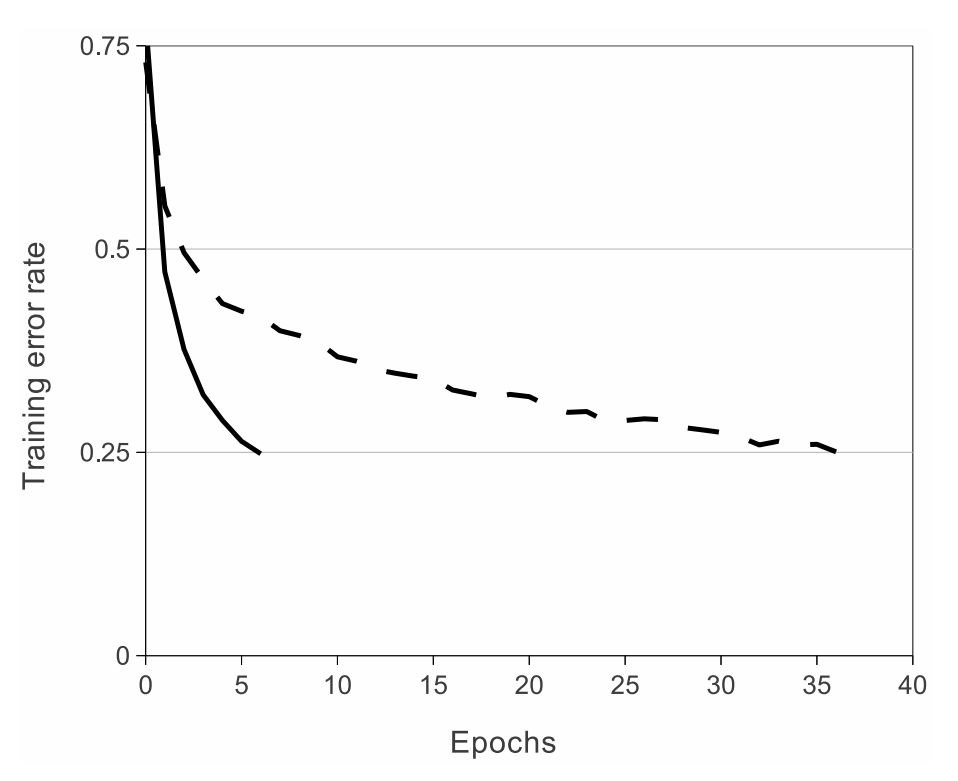
\includegraphics[width=0.7\linewidth]{img/01-01} \end{center}

Figure 1: A four-layer convolutional neural network with ReLUs \textbf{(solid line)} reaches a 25\% training error rate on CIFAR-10 six times faster than an equivalent network with tanh neurons \textbf{(dashed line)}. The learning rates for each network were chosen independently to make training as fast as possible. No regularization of any kind was employed. The magnitude of the effect demonstrated here varies with network architecture, but networks with ReLUs consistently learn several times faster than equivalents with saturating neurons.

\hypertarget{training-on-multiple-gpus}{%
\subsection{Training on Multiple GPUs}\label{training-on-multiple-gpus}}

A single GTX 580 GPU has only 3GB of memory, which limits the maximum size of the networks that can be trained on it. It turns out that 1.2 million training examples are enough to train networks which are too big to fit on one GPU. Therefore we spread the net across two GPUs. Current GPUs are particularly well-suited to cross-GPU parallelization, as they are able to read from and write to one another's memory directly, without going through host machine memory. The parallelization scheme that we employ essentially puts half of the kernels (or neurons) on each GPU, with one additional trick: the GPUs communicate only in certain layers. This means that, for example, the kernels of layer 3 take input from all kernel maps in layer 2. However, kernels in layer 4 take input only from those kernel maps in layer 3 which reside on the same GPU. Choosing the pattern of connectivity is a problem for cross-validation, but this allows us to precisely tune the amount of communication until it is an acceptable fraction of the amount of computation.

The resultant architecture is somewhat similar to that of the ``columnar'' CNN employed by Cire¸san et al.~{[}5{]}, except that our columns are not independent (see Figure 2). This scheme reduces our top-1 and top-5 error rates by 1.7\% and 1.2\%, respectively, as compared with a net with half as many kernels in each convolutional layer trained on one GPU. The two-GPU net takes slightly less time to train than the one-GPU \(net^2\).

\hypertarget{local-response-normalization}{%
\subsection{Local Response Normalization}\label{local-response-normalization}}

ReLUs have the desirable property that they do not require input normalization to prevent them from saturating. If at least some training examples produce a positive input to a ReLU, learning will happen in that neuron. However, we still find that the following local normalization scheme aids generalization. Denoting by \(a^i_{x,y}\) the activity of a neuron computed by applying kernel i at position \((x, y)\) and then applying the ReLU nonlinearity, the response-normalized activity \(b^i_{x,y}\) is given by the expression

\[b^i_{x,y} = a^i_{x,y}/\bigg(k+\alpha\sum\limits_{j=max(0,i-n/2)}^{min(N-1,i+n/2)}(a_{x,y}^j)^2\bigg)^\beta\]

where the sum runs over n ``adjacent'' kernel maps at the same spatial position, and N is the total number of kernels in the layer. The ordering of the kernel maps is of course arbitrary and determined before training begins. This sort of response normalization implements a form of lateral inhibition inspired by the type found in real neurons, creating competition for big activities amongst neuron outputs computed using different kernels. The constants \(k\), \(n\), \(\alpha\), and \(\beta\) are hyper-parameters whose values are determined using a validation set; we used \(k = 2\), \(n = 5\), \(\alpha = 10^−4\), and \(\beta = 0.75\). We applied this normalization after applying the ReLU nonlinearity in certain layers (see Section 3.5).

This scheme bears some resemblance to the local contrast normalization scheme of Jarrett et al.~{[}11{]}, but ours would be more correctly termed ``brightness normalization'', since we do not subtract the mean activity. Response normalization reduces our top-1 and top-5 error rates by 1.4\% and 1.2\%, respectively. We also verified the effectiveness of this scheme on the CIFAR-10 dataset: a four-layer CNN achieved a 13\% test error rate without normalization and 11\% with \(normalization^3\).

\hypertarget{overlapping-pooling}{%
\subsection{Overlapping Pooling}\label{overlapping-pooling}}

Pooling layers in CNNs summarize the outputs of neighboring groups of neurons in the same kernel map. Traditionally, the neighborhoods summarized by adjacent pooling units do not overlap (e.g., {[}17, 11, 4{]}). To be more precise, a pooling layer can be thought of as consisting of a grid of pooling units spaced s pixels apart, each summarizing a neighborhood of size \(z × z\) centered at the location of the pooling unit. If we set \(s = z\), we obtain traditional local pooling as commonly employed in CNNs. If we set \(s < z\), we obtain overlapping pooling. This is what we use throughout our network, with \(s = 2\) and \(z = 3\). This scheme reduces the top-1 and top-5 error rates by 0.4\% and 0.3\%, respectively, as compared with the non-overlapping scheme \(s = 2\), \(z = 2\), which produces output of equivalent dimensions. We generally observe during training that models with overlapping pooling find it slightly more difficult to overfit.

\hypertarget{overall-architecture}{%
\subsection{Overall Architecture}\label{overall-architecture}}

Now we are ready to describe the overall architecture of our CNN. As depicted in Figure 2, the net contains eight layers with weights; the first five are convolutional and the remaining three are fully-connected. The output of the last fully-connected layer is fed to a 1000-way softmax which produces a distribution over the 1000 class labels. Our network maximizes the multinomial logistic regression objective, which is equivalent to maximizing the average across training cases of the log-probability of the correct label under the prediction distribution.

The kernels of the second, fourth, and fifth convolutional layers are connected only to those kernel maps in the previous layer which reside on the same GPU (see Figure 2). The kernels of the third convolutional layer are connected to all kernel maps in the second layer. The neurons in the fully connected layers are connected to all neurons in the previous layer. Response-normalization layers follow the first and second convolutional layers. Max-pooling layers, of the kind described in Section 3.4, follow both response-normalization layers as well as the fifth convolutional layer. The ReLU non-linearity is applied to the output of every convolutional and fully-connected layer.

\begin{center}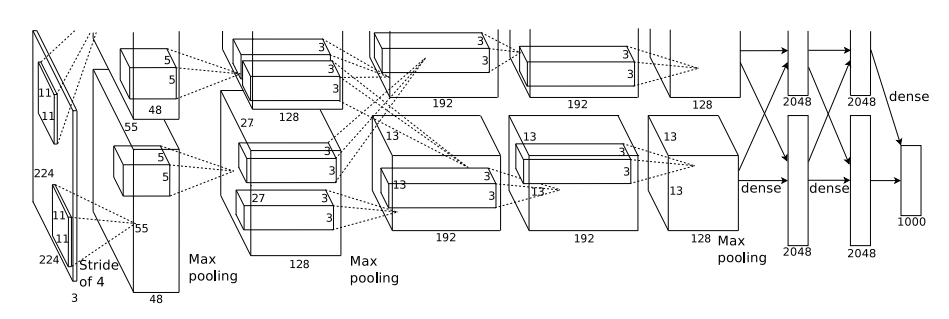
\includegraphics[width=0.7\linewidth]{img/01-02} \end{center}

Figure 2: An illustration of the architecture of our CNN, explicitly showing the delineation of responsibilities between the two GPUs. One GPU runs the layer-parts at the top of the figure while the other runs the layer-parts at the bottom. The GPUs communicate only at certain layers. The network's input is 150,528-dimensional, and the number of neurons in the network's remaining layers is given by 253,440--186,624--64,896--64,896--43,264--4096--4096--1000.

The first convolutional layer filters the 224×224×3 input image with 96 kernels of size 11×11×3 with a stride of 4 pixels (this is the distance between the receptive field centers of neighboring neurons in a kernel map). The second convolutional layer takes as input the (response-normalized and pooled) output of the first convolutional layer and filters it with 256 kernels of size 5 × 5 × 48. The third, fourth, and fifth convolutional layers are connected to one another without any intervening pooling or normalization layers. The third convolutional layer has 384 kernels of size 3 × 3 × 256 connected to the (normalized, pooled) outputs of the second convolutional layer. The fourth convolutional layer has 384 kernels of size 3 × 3 × 192 , and the fifth convolutional layer has 256 kernels of size 3 × 3 × 192. The fully-connected layers have 4096 neurons each.

\hypertarget{reducing-overfitting}{%
\section{Reducing Overfitting}\label{reducing-overfitting}}

Our neural network architecture has 60 million parameters. Although the 1000 classes of ILSVRC make each training example impose 10 bits of constraint on the mapping from image to label, this turns out to be insufficient to learn so many parameters without considerable overfitting. Below, we describe the two primary ways in which we combat overfitting.

\hypertarget{data-augmentation}{%
\subsection{Data Augmentation}\label{data-augmentation}}

The easiest and most common method to reduce overfitting on image data is to artificially enlarge the dataset using label-preserving transformations (e.g., {[}25, 4, 5{]}). We employ two distinct forms of data augmentation, both of which allow transformed images to be produced from the original images with very little computation, so the transformed images do not need to be stored on disk. In our implementation, the transformed images are generated in Python code on the CPU while the GPU is training on the previous batch of images. So these data augmentation schemes are, in effect, computationally free.

The first form of data augmentation consists of generating image translations and horizontal reflections. We do this by extracting random 224 × 224 patches (and their horizontal reflections) from the 256×256 images and training our network on these extracted \(patches^4\) . This increases the size of our training set by a factor of 2048, though the resulting training examples are, of course, highly inter dependent. Without this scheme, our network suffers from substantial overfitting, which would have forced us to use much smaller networks. At test time, the network makes a prediction by extracting five 224 × 224 patches (the four corner patches and the center patch) as well as their horizontal reflections (hence ten patches in all), and averaging the predictions made by the network's softmax layer on the ten patches.

The second form of data augmentation consists of altering the intensities of the RGB channels in training images. Specifically, we perform PCA on the set of RGB pixel values throughout the ImageNet training set. To each training image, we add multiples of the found principal components, with magnitudes proportional to the corresponding eigenvalues times a random variable drawn from a Gaussian with mean zero and standard deviation 0.1. Therefore to each RGB image pixel \(I_{xy} = \left[ \begin{matrix} I^R_{xy} & I^G_{xy} & I^B_{xy} \end{matrix} \right]^T\) we add the following quantity:

\[
\left[ \begin{matrix} P_1 & P_2 & P_3 \end{matrix} \right]\left[ \begin{matrix} \alpha_1\lambda_1 & \alpha_2\lambda_2 & \alpha_3\lambda_3 \end{matrix} \right]^T
\]

where \(P_i\) and \(\lambda_i\) are \(i\)th eigenvector and eigenvalue of the 3 × 3 covariance matrix of RGB pixel values, respectively, and \(\alpha_i\) is the aforementioned random variable. Each \(\alpha_i\) is drawn only once for all the pixels of a particular training image until that image is used for training again, at which point it is re-drawn. This scheme approximately captures an important property of natural images, namely, that object identity is invariant to changes in the intensity and color of the illumination. This scheme reduces the top-1 error rate by over 1\%.

\hypertarget{dropout}{%
\subsection{Dropout}\label{dropout}}

Combining the predictions of many different models is a very successful way to reduce test errors {[}1, 3{]}, but it appears to be too expensive for big neural networks that already take several days to train. There is, however, a very efficient version of model combination that only costs about a factor of two during training. The recently-introduced technique, called ``dropout'' {[}10{]}, consists of setting to zero the output of each hidden neuron with probability 0.5. The neurons which are ``dropped out'' in this way do not contribute to the forward pass and do not participate in back-propagation. So every time an input is presented, the neural network samples a different architecture, but all these architectures share weights. This technique reduces complex co-adaptations of neurons, since a neuron cannot rely on the presence of particular other neurons. It is, therefore, forced to learn more robust features that are useful in conjunction with many different random subsets of the other neurons. At test time, we use all the neurons but multiply their outputs by 0.5, which is a reasonable approximation to taking the geometric mean of the predictive distributions produced by the exponentially-many dropout networks.

We use dropout in the first two fully-connected layers of Figure 2. Without dropout, our network exhibits substantial overfitting. Dropout roughly doubles the number of iterations required to converge.

\hypertarget{details-of-learning}{%
\section{Details of learning}\label{details-of-learning}}

We trained our models using stochastic gradient descent with a batch size of 128 examples, momentum of 0.9, and weight decay of 0.0005. We found that this small amount of weight decay was important for the model to learn. In other words, weight decay here is not merely a regularizer: it reduces the model's training error. The update rule for weight \(w\) was

\[
v_{i+1} := 0.9 \cdot v_i - 0.0005 \cdot \epsilon \cdot w_i - \epsilon \cdot \left\langle \frac{\partial L}{\partial w} \mid_{w_i} \right\rangle _{D_i}
\]
\[
w_{i+1} := w_i + v_{i+1}
\]

where \(i\) is the iteration index, \(v\) is the momentum variable, \(\epsilon\) is the learning rate, and \(\left\langle \frac{\partial L}{\partial w} \mid_{w_i} \right\rangle _{D_i}\) is the average over the \(i\)th batch \(D_i\) of the derivative of the objective with respect to \(w\), evaluated at \(w_i\).

\begin{center}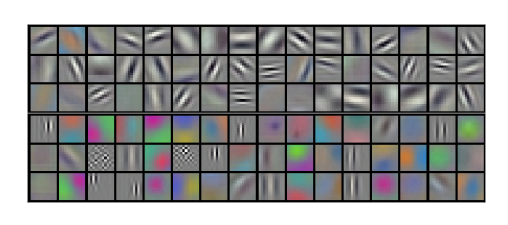
\includegraphics[width=0.7\linewidth]{img/01-03} \end{center}

Figure 3: 96 convolutional kernels of size 11×11×3 learned by the first convolutional layer on the 224×224×3 input images. The top 48 kernels were learned on GPU 1 while the bottom 48 kernels were learned on GPU 2. See Section 6.1 for details.

We initialized the weights in each layer from a zero-mean Gaussian distribution with standard deviation 0.01. We initialized the neuron biases in the second, fourth, and fifth convolutional layers, as well as in the fully-connected hidden layers, with the constant 1. This initialization accelerates the early stages of learning by providing the ReLUs with positive inputs. We initialized the neuron biases in the remaining layers with the constant 0.

We used an equal learning rate for all layers, which we adjusted manually throughout training. The heuristic which we followed was to divide the learning rate by 10 when the validation error rate stopped improving with the current learning rate. The learning rate was initialized at 0.01 and reduced three times prior to termination. We trained the network for roughly 90 cycles through the training set of 1.2 million images, which took five to six days on two NVIDIA GTX 580 3GB GPUs.

\hypertarget{results}{%
\section{Results}\label{results}}

Our results on ILSVRC-2010 are summarized in Table 1. Our network achieves top-1 and top-5 test set error rates of 37.5\% and \(17.0%^5
\). The best performance achieved during the ILSVRC-2010 competition was 47.1\% and 28.2\% with an approach that averages the predictions produced from six sparse-coding models trained on different features {[}2{]}, and since then the best published results are 45.7\% and 25.7\% with an approach that averages the predictions of two classifiers trained on Fisher Vectors (FVs) computed from two types of densely-sampled features {[}24{]}.

\begin{longtable}[]{@{}lll@{}}
\toprule
\textbf{Model} & \textbf{Top-1} & \textbf{Top-5}\tabularnewline
\midrule
\endhead
Sparse coding {[}2{]} & 47.1\% & 28.2\%\tabularnewline
SIFT + FVs {[}24{]} & 45.7\% & 25.7\%\tabularnewline
CNN & \textbf{37.5} & \textbf{17.0\%}\tabularnewline
\bottomrule
\end{longtable}

Table 1: Comparison of results on ILSVRC-2010 test set. In italics are best results achieved by others.

We also entered our model in the ILSVRC-2012 competition and report our results in Table 2. Since the ILSVRC-2012 test set labels are not publicly available, we cannot report test error rates for all the models that we tried. In the remainder of this paragraph, we use validation and test error rates interchangeably because in our experience they do not differ by more than 0.1\% (see Table 2). The CNN described in this paper achieves a top-5 error rate of 18.2\%. Averaging the predictions of five similar CNNs gives an error rate of 16.4\%. Training one CNN, with an extra sixth convolutional layer over the last pooling layer, to classify the entire ImageNet Fall 2011 release (15M images, 22K categories), and then ``fine-tuning'' it on ILSVRC-2012 gives an error rate of 16.6\%. Averaging the predictions of two CNNs that were pre-trained on the entire Fall 2011 release with the aforementioned five CNNs gives an error rate of 15.3\%. The second-best contest entry achieved an error rate of 26.2\% with an approach that averages the predictions of several classifiers trained on FVs computed from different types of densely-sampled features {[}7{]}.

\begin{longtable}[]{@{}llll@{}}
\toprule
\textbf{Model} & \textbf{Top-1(val)} & \textbf{Top-5(val)} & \textbf{Top-5(test)}\tabularnewline
\midrule
\endhead
SIFT + FVs {[}7{]} & - & - & 26.2\%\tabularnewline
1 CNN & 40.7\% & 18.2\% & -\tabularnewline
5 CNNs & 38.1\% & 16.4\% & \textbf{16.4\%}\tabularnewline
1 CNN* & 39.0\% & 16.6\% & -\tabularnewline
7 CNNs* & 36.7\% & 15.4\% & \textbf{15.3\%}\tabularnewline
\bottomrule
\end{longtable}

Table 2: Comparison of error rates on ILSVRC-2012 validation and test sets. In italics are best results achieved by others. Models with an asterisk* were ``pre-trained'' to classify the entire ImageNet 2011 Fall release. See Section 6 for details.

Finally, we also report our error rates on the Fall 2009 version of ImageNet with 10,184 categories and 8.9 million images. On this dataset we follow the convention in the literature of using half of the images for training and half for testing. Since there is no established test set, our split necessarily differs from the splits used by previous authors, but this does not affect the results appreciably. Our top-1 and top-5 error rates on this dataset are 67.4\% and 40.9\%, attained by the net described above but with an additional, sixth convolutional layer over the last pooling layer. The best published results on this dataset are 78.1\% and 60.9\% {[}19{]}.

\hypertarget{qualitative-evaluations}{%
\subsection{Qualitative Evaluations}\label{qualitative-evaluations}}

Figure 3 shows the convolutional kernels learned by the network's two data-connected layers. The network has learned a variety of frequency- and orientation-selective kernels, as well as various colored blobs. Notice the specialization exhibited by the two GPUs, a result of the restricted connectivity described in Section 3.5. The kernels on GPU 1 are largely color-agnostic, while the kernels on on GPU 2 are largely color-specific. This kind of specialization occurs during every run and is independent of any particular random weight initialization (modulo a renumbering of the GPUs).

\begin{center}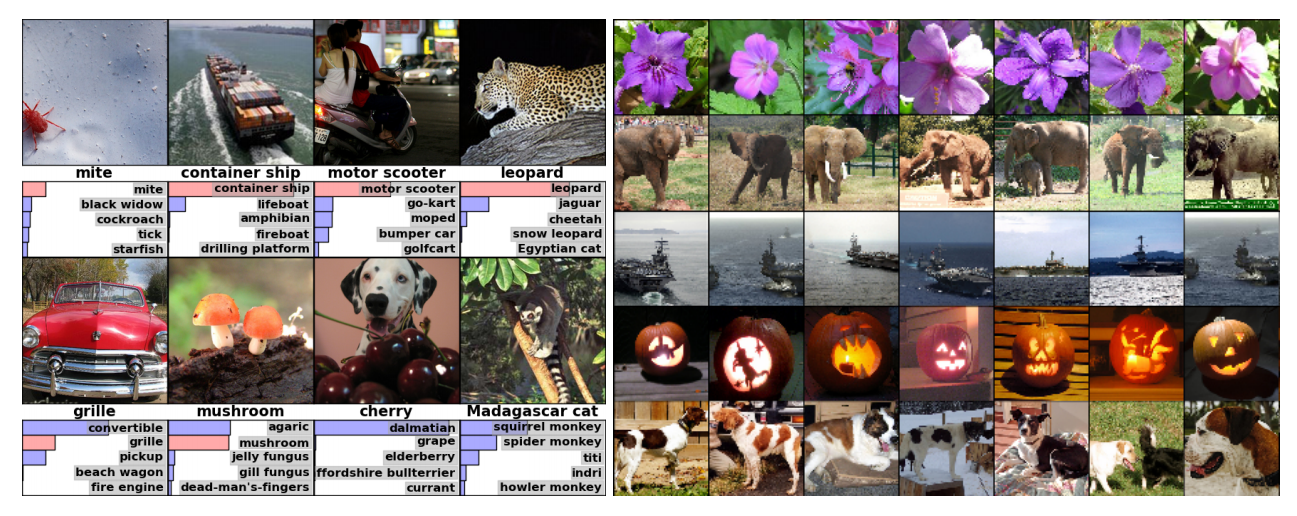
\includegraphics[width=0.7\linewidth]{img/01-04} \end{center}

Figure 4: (Left) Eight ILSVRC-2010 test images and the five labels considered most probable by our model. The correct label is written under each image, and the probability assigned to the correct label is also shown with a red bar (if it happens to be in the top 5). (Right) Five ILSVRC-2010 test images in the first column. The remaining columns show the six training images that produce feature vectors in the last hidden layer with the smallest Euclidean distance from the feature vector for the test image.

In the left panel of Figure 4 we qualitatively assess what the network has learned by computing its top-5 predictions on eight test images. Notice that even off-center objects, such as the mite in the top-left, can be recognized by the net. Most of the top-5 labels appear reasonable. For example, only other types of cat are considered plausible labels for the leopard. In some cases (grille, cherry) there is genuine ambiguity about the intended focus of the photograph.

Another way to probe the network's visual knowledge is to consider the feature activations induced by an image at the last, 4096-dimensional hidden layer. If two images produce feature activation vectors with a small Euclidean separation, we can say that the higher levels of the neural network consider them to be similar. Figure 4 shows five images from the test set and the six images from the training set that are most similar to each of them according to this measure. Notice that at the pixel level, the retrieved training images are generally not close in L2 to the query images in the first column. For example, the retrieved dogs and elephants appear in a variety of poses. We present the results for many more test images in the supplementary material.

Computing similarity by using Euclidean distance between two 4096-dimensional, real-valued vectors is inefficient, but it could be made efficient by training an auto-encoder to compress these vectors to short binary codes. This should produce a much better image retrieval method than applying auto-encoders to the raw pixels {[}14{]}, which does not make use of image labels and hence has a tendency to retrieve images with similar patterns of edges, whether or not they are semantically similar

\hypertarget{discussion}{%
\section{Discussion}\label{discussion}}

Our results show that a large, deep convolutional neural network is capable of achieving record-breaking results on a highly challenging dataset using purely supervised learning. It is notable that our network's performance degrades if a single convolutional layer is removed. For example, removing any of the middle layers results in a loss of about 2\% for the top-1 performance of the network. So the depth really is important for achieving our results.

To simplify our experiments, we did not use any unsupervised pre-training even though we expect that it will help, especially if we obtain enough computational power to significantly increase the size of the network without obtaining a corresponding increase in the amount of labeled data. Thus far, our results have improved as we have made our network larger and trained it longer but we still have many orders of magnitude to go in order to match the infero-temporal pathway of the human visual system. Ultimately we would like to use very large and deep convolutional nets on video sequences where the temporal structure provides very helpful information that is missing or far less obvious in static images.

\hypertarget{ux7ecfux5178ux6df1ux5ea6ux5b66ux4e60ux7f51ux7edcux6a21ux578b}{%
\chapter{经典深度学习网络模型}\label{ux7ecfux5178ux6df1ux5ea6ux5b66ux4e60ux7f51ux7edcux6a21ux578b}}

\hypertarget{lenet-5}{%
\section{LeNet-5}\label{lenet-5}}

\hypertarget{ux6a21ux578bux4ecbux7ecd}{%
\subsection{模型介绍}\label{ux6a21ux578bux4ecbux7ecd}}

LeNet-5是由\(LeCun\) 提出的一种用于识别手写数字和机器印刷字符的卷积神经网络(Convolutional Neural Network,CNN)\(^{[1]}\),其命名来源于作者\(LeCun\)的名字,5则是其研究成果的代号,在LeNet-5之前还有LeNet-4和LeNet-1鲜为人知。LeNet-5阐述了图像中像素特征之间的相关性能够由参数共享的卷积操作所提取,同时使用卷积、下采样(池化)和非线性映射这样的组合结构,是当前流行的大多数深度图像识别网络的基础。

\hypertarget{ux6a21ux578bux7ed3ux6784}{%
\subsection{模型结构}\label{ux6a21ux578bux7ed3ux6784}}

\begin{center}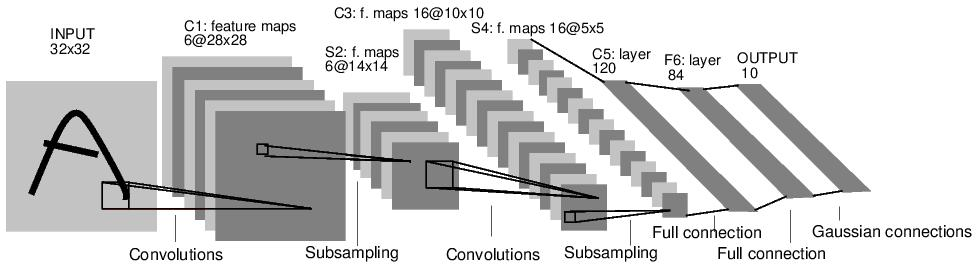
\includegraphics[width=0.7\linewidth]{img/02-01} \end{center}

LeNet-5一共包含7层(输入层不作为网络结构),分别由2个卷积层、2个下采样层和3个全连接层组成,网络的参数配置如下表所示,其中下采样层和全连接层的核尺寸分别代表采样范围和连接矩阵的尺寸(如卷积核尺寸中的\(“5\times5\times1/1,6”\)表示核大小为\(5\times5\times1\)、步长为\(1\)且核个数为6的卷积核)。

LeNet-5网络参数配置:

\begin{longtable}[]{@{}ccccc@{}}
\toprule
\begin{minipage}[b]{0.12\columnwidth}\centering
网络层\strut
\end{minipage} & \begin{minipage}[b]{0.16\columnwidth}\centering
输入尺寸\strut
\end{minipage} & \begin{minipage}[b]{0.19\columnwidth}\centering
核尺寸\strut
\end{minipage} & \begin{minipage}[b]{0.16\columnwidth}\centering
输出尺寸\strut
\end{minipage} & \begin{minipage}[b]{0.24\columnwidth}\centering
可训练参数量\strut
\end{minipage}\tabularnewline
\midrule
\endhead
\begin{minipage}[t]{0.12\columnwidth}\centering
卷积层\(C_1\)\strut
\end{minipage} & \begin{minipage}[t]{0.16\columnwidth}\centering
\(32\times32\times1\)\strut
\end{minipage} & \begin{minipage}[t]{0.19\columnwidth}\centering
\(5\times5\times1/1,6\)\strut
\end{minipage} & \begin{minipage}[t]{0.16\columnwidth}\centering
\(28\times28\times6\)\strut
\end{minipage} & \begin{minipage}[t]{0.24\columnwidth}\centering
\((5\times5\times1+1)\times6\)\strut
\end{minipage}\tabularnewline
\begin{minipage}[t]{0.12\columnwidth}\centering
下采样层\(S_2\)\strut
\end{minipage} & \begin{minipage}[t]{0.16\columnwidth}\centering
\(28\times28\times6\)\strut
\end{minipage} & \begin{minipage}[t]{0.19\columnwidth}\centering
\(2\times2/2\)\strut
\end{minipage} & \begin{minipage}[t]{0.16\columnwidth}\centering
\(14\times14\times6\)\strut
\end{minipage} & \begin{minipage}[t]{0.24\columnwidth}\centering
\((1+1)\times6\) \(^*\)\strut
\end{minipage}\tabularnewline
\begin{minipage}[t]{0.12\columnwidth}\centering
卷积层\(C_3\)\strut
\end{minipage} & \begin{minipage}[t]{0.16\columnwidth}\centering
\(14\times14\times6\)\strut
\end{minipage} & \begin{minipage}[t]{0.19\columnwidth}\centering
\(5\times5\times6/1,16\)\strut
\end{minipage} & \begin{minipage}[t]{0.16\columnwidth}\centering
\(10\times10\times16\)\strut
\end{minipage} & \begin{minipage}[t]{0.24\columnwidth}\centering
\(1516^*\)\strut
\end{minipage}\tabularnewline
\begin{minipage}[t]{0.12\columnwidth}\centering
下采样层\(S_4\)\strut
\end{minipage} & \begin{minipage}[t]{0.16\columnwidth}\centering
\(10\times10\times16\)\strut
\end{minipage} & \begin{minipage}[t]{0.19\columnwidth}\centering
\(2\times2/2\)\strut
\end{minipage} & \begin{minipage}[t]{0.16\columnwidth}\centering
\(5\times5\times16\)\strut
\end{minipage} & \begin{minipage}[t]{0.24\columnwidth}\centering
\((1+1)\times16\)\strut
\end{minipage}\tabularnewline
\begin{minipage}[t]{0.12\columnwidth}\centering
卷积层\(C_5\)\(^*\)\strut
\end{minipage} & \begin{minipage}[t]{0.16\columnwidth}\centering
\(5\times5\times16\)\strut
\end{minipage} & \begin{minipage}[t]{0.19\columnwidth}\centering
\(5\times5\times16/1,120\)\strut
\end{minipage} & \begin{minipage}[t]{0.16\columnwidth}\centering
\(1\times1\times120\)\strut
\end{minipage} & \begin{minipage}[t]{0.24\columnwidth}\centering
\((5\times5\times16+1)\times120\)\strut
\end{minipage}\tabularnewline
\begin{minipage}[t]{0.12\columnwidth}\centering
全连接层\(F_6\)\strut
\end{minipage} & \begin{minipage}[t]{0.16\columnwidth}\centering
\(1\times1\times120\)\strut
\end{minipage} & \begin{minipage}[t]{0.19\columnwidth}\centering
\(120\times84\)\strut
\end{minipage} & \begin{minipage}[t]{0.16\columnwidth}\centering
\(1\times1\times84\)\strut
\end{minipage} & \begin{minipage}[t]{0.24\columnwidth}\centering
\((120+1)\times84\)\strut
\end{minipage}\tabularnewline
\begin{minipage}[t]{0.12\columnwidth}\centering
输出层\strut
\end{minipage} & \begin{minipage}[t]{0.16\columnwidth}\centering
\(1\times1\times84\)\strut
\end{minipage} & \begin{minipage}[t]{0.19\columnwidth}\centering
\(84\times10\)\strut
\end{minipage} & \begin{minipage}[t]{0.16\columnwidth}\centering
\(1\times1\times10\)\strut
\end{minipage} & \begin{minipage}[t]{0.24\columnwidth}\centering
\((84+1)\times10\)\strut
\end{minipage}\tabularnewline
\bottomrule
\end{longtable}

\(^*\) 在LeNet中,下采样操作和池化操作类似,但是在得到采样结果后会乘以一个系数和加上一个偏置项,所以下采样的参数个数是\((1+1)\times6\)而不是零。

\(^*\) \(C_3\)卷积层可训练参数并未直接连接\(S_2\)中所有的特征图(Feature Map),而是采用如下图所示的采样特征方式进行连接(稀疏连接),生成的16个通道特征图中分别按照相邻3个特征图、相邻4个特征图、非相邻4个特征图和全部6个特征图进行映射,得到的参数个数计算公式为\(6\times(25\times3+1)+6\times(25\times4+1)+3\times(25\times4+1)+1\times(25\times6+1)=1516\),在原论文中解释了使用这种采样方式原因包含两点:限制了连接数不至于过大(当年的计算能力比较弱);强制限定不同特征图的组合可以使映射得到的特征图学习到不同的特征模式。

\(S_2\)与\(C_3\)之间的特征图稀疏连接

\begin{center}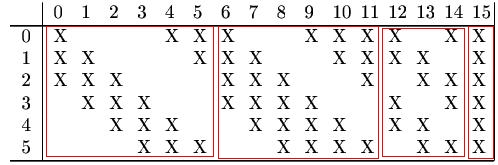
\includegraphics[width=0.7\linewidth]{img/02-02} \end{center}

\(^*\) \(C_5\)卷积层显示为全连接层,原论文中解释这里实际采用的是卷积操作,只是刚好在\(5\times5\)卷积后尺寸被压缩为\(1\times1\),输出结果看起来和全连接很相似。

\hypertarget{ux6a21ux578bux7279ux6027}{%
\subsection{模型特性}\label{ux6a21ux578bux7279ux6027}}

\begin{itemize}
\tightlist
\item
  卷积网络使用一个3层的序列组合:卷积、下采样(池化)、非线性映射(LeNet-5最重要的特性,奠定了目前深层卷积网络的基础)
\item
  使用卷积提取空间特征
\item
  使用映射的空间均值进行下采样
\item
  使用\(tanh\)或\(sigmoid\)进行非线性映射
\item
  多层神经网络(MLP)作为最终的分类器
\item
  层间的稀疏连接矩阵以避免巨大的计算开销
\end{itemize}

\hypertarget{alexnet}{%
\section{AlexNet}\label{alexnet}}

\hypertarget{ux6a21ux578bux4ecbux7ecd-1}{%
\subsection{模型介绍}\label{ux6a21ux578bux4ecbux7ecd-1}}

AlexNet是由\emph{Alex Krizhevsky}提出的首个应用于图像分类的深层卷积神经网络,该网络在2012年ILSVRC(ImageNet Large Scale Visual Recognition Competition)图像分类竞赛中以15.3\%的top-5测试错误率赢得第一名。AlexNet使用GPU代替CPU进行运算,使得在可接受的时间范围内模型结构能够更加复杂,它的出现证明了深层卷积神经网络在复杂模型下的有效性,使CNN在计算机视觉中流行开来,直接或间接地引发了深度学习的热潮。

\hypertarget{ux6a21ux578bux7ed3ux6784-1}{%
\subsection{模型结构}\label{ux6a21ux578bux7ed3ux6784-1}}

\begin{center}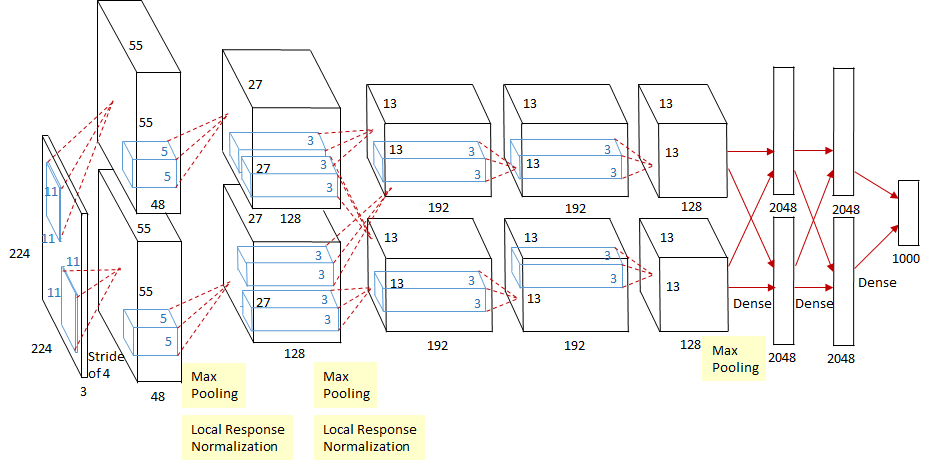
\includegraphics[width=0.7\linewidth]{img/02-03} \end{center}

除去下采样(池化层)和局部响应规范化操作(Local Responsible Normalization, LRN),AlexNet一共包含8层,前5层由卷积层组成,而剩下的3层为全连接层。网络结构分为上下两层,分别对应两个GPU的操作过程,除了中间某些层(\(C_3\)卷积层和\(F_{6-8}\)全连接层会有GPU间的交互),其他层两个GPU分别计算结果。最后一层全连接层的输出作为\(softmax\)的输入,得到1000个图像分类标签对应的概率值。除去GPU并行结构的设计,AlexNet网络结构与LeNet十分相似,其网络的参数配置如表所示。

\begin{longtable}[]{@{}ccccc@{}}
\toprule
\begin{minipage}[b]{0.17\columnwidth}\centering
网络层\strut
\end{minipage} & \begin{minipage}[b]{0.17\columnwidth}\centering
输入尺寸\strut
\end{minipage} & \begin{minipage}[b]{0.17\columnwidth}\centering
核尺寸\strut
\end{minipage} & \begin{minipage}[b]{0.17\columnwidth}\centering
输出尺寸\strut
\end{minipage} & \begin{minipage}[b]{0.17\columnwidth}\centering
可训练参数量\strut
\end{minipage}\tabularnewline
\midrule
\endhead
\begin{minipage}[t]{0.17\columnwidth}\centering
卷积层\(C_1\) \(^*\)\strut
\end{minipage} & \begin{minipage}[t]{0.17\columnwidth}\centering
\(224\times224\times3\)\strut
\end{minipage} & \begin{minipage}[t]{0.17\columnwidth}\centering
\(11\times11\times3/4,48(\times2_{GPU})\)\strut
\end{minipage} & \begin{minipage}[t]{0.17\columnwidth}\centering
\(55\times55\times48(\times2_{GPU})\)\strut
\end{minipage} & \begin{minipage}[t]{0.17\columnwidth}\centering
\((11\times11\times3+1)\times48\times2\)\strut
\end{minipage}\tabularnewline
\begin{minipage}[t]{0.17\columnwidth}\centering
下采样层\(S_{max}\)\(^*\)\strut
\end{minipage} & \begin{minipage}[t]{0.17\columnwidth}\centering
\(55\times55\times48(\times2_{GPU})\)\strut
\end{minipage} & \begin{minipage}[t]{0.17\columnwidth}\centering
\(3\times3/2(\times2_{GPU})\)\strut
\end{minipage} & \begin{minipage}[t]{0.17\columnwidth}\centering
\(27\times27\times48(\times2_{GPU})\)\strut
\end{minipage} & \begin{minipage}[t]{0.17\columnwidth}\centering
0\strut
\end{minipage}\tabularnewline
\begin{minipage}[t]{0.17\columnwidth}\centering
卷积层\(C_2\)\strut
\end{minipage} & \begin{minipage}[t]{0.17\columnwidth}\centering
\(27\times27\times48(\times2_{GPU})\)\strut
\end{minipage} & \begin{minipage}[t]{0.17\columnwidth}\centering
\(5\times5\times48/1,128(\times2_{GPU})\)\strut
\end{minipage} & \begin{minipage}[t]{0.17\columnwidth}\centering
\(27\times27\times128(\times2_{GPU})\)\strut
\end{minipage} & \begin{minipage}[t]{0.17\columnwidth}\centering
\((5\times5\times48+1)\times128\times2\)\strut
\end{minipage}\tabularnewline
\begin{minipage}[t]{0.17\columnwidth}\centering
下采样层\(S_{max}\)\strut
\end{minipage} & \begin{minipage}[t]{0.17\columnwidth}\centering
\(27\times27\times128(\times2_{GPU})\)\strut
\end{minipage} & \begin{minipage}[t]{0.17\columnwidth}\centering
\(3\times3/2(\times2_{GPU})\)\strut
\end{minipage} & \begin{minipage}[t]{0.17\columnwidth}\centering
\(13\times13\times128(\times2_{GPU})\)\strut
\end{minipage} & \begin{minipage}[t]{0.17\columnwidth}\centering
0\strut
\end{minipage}\tabularnewline
\begin{minipage}[t]{0.17\columnwidth}\centering
卷积层\(C_3\) \(^*\)\strut
\end{minipage} & \begin{minipage}[t]{0.17\columnwidth}\centering
\(13\times13\times128\times2_{GPU}\)\strut
\end{minipage} & \begin{minipage}[t]{0.17\columnwidth}\centering
\(3\times3\times256/1,192(\times2_{GPU})\)\strut
\end{minipage} & \begin{minipage}[t]{0.17\columnwidth}\centering
\(13\times13\times192(\times2_{GPU})\)\strut
\end{minipage} & \begin{minipage}[t]{0.17\columnwidth}\centering
\((3\times3\times256+1)\times192\times2\)\strut
\end{minipage}\tabularnewline
\begin{minipage}[t]{0.17\columnwidth}\centering
卷积层\(C_4\)\strut
\end{minipage} & \begin{minipage}[t]{0.17\columnwidth}\centering
\(13\times13\times192(\times2_{GPU})\)\strut
\end{minipage} & \begin{minipage}[t]{0.17\columnwidth}\centering
\(3\times3\times192/1,192(\times2_{GPU})\)\strut
\end{minipage} & \begin{minipage}[t]{0.17\columnwidth}\centering
\(13\times13\times192(\times2_{GPU})\)\strut
\end{minipage} & \begin{minipage}[t]{0.17\columnwidth}\centering
\((3\times3\times192+1)\times192\times2\)\strut
\end{minipage}\tabularnewline
\begin{minipage}[t]{0.17\columnwidth}\centering
卷积层\(C_5\)\strut
\end{minipage} & \begin{minipage}[t]{0.17\columnwidth}\centering
\(13\times13\times192(\times2_{GPU})\)\strut
\end{minipage} & \begin{minipage}[t]{0.17\columnwidth}\centering
\(3\times3\times192/1,128(\times2_{GPU})\)\strut
\end{minipage} & \begin{minipage}[t]{0.17\columnwidth}\centering
\(13\times13\times128(\times2_{GPU})\)\strut
\end{minipage} & \begin{minipage}[t]{0.17\columnwidth}\centering
\((3\times3\times192+1)\times128\times2\)\strut
\end{minipage}\tabularnewline
\begin{minipage}[t]{0.17\columnwidth}\centering
下采样层\(S_{max}\)\strut
\end{minipage} & \begin{minipage}[t]{0.17\columnwidth}\centering
\(13\times13\times128(\times2_{GPU})\)\strut
\end{minipage} & \begin{minipage}[t]{0.17\columnwidth}\centering
\(3\times3/2(\times2_{GPU})\)\strut
\end{minipage} & \begin{minipage}[t]{0.17\columnwidth}\centering
\(6\times6\times128(\times2_{GPU})\)\strut
\end{minipage} & \begin{minipage}[t]{0.17\columnwidth}\centering
0\strut
\end{minipage}\tabularnewline
\begin{minipage}[t]{0.17\columnwidth}\centering
全连接层\(F_6\) \(^*\)\strut
\end{minipage} & \begin{minipage}[t]{0.17\columnwidth}\centering
\(6\times6\times128\times2_{GPU}\)\strut
\end{minipage} & \begin{minipage}[t]{0.17\columnwidth}\centering
\(9216\times2048(\times2_{GPU})\)\strut
\end{minipage} & \begin{minipage}[t]{0.17\columnwidth}\centering
\(1\times1\times2048(\times2_{GPU})\)\strut
\end{minipage} & \begin{minipage}[t]{0.17\columnwidth}\centering
\((9216+1)\times2048\times2\)\strut
\end{minipage}\tabularnewline
\begin{minipage}[t]{0.17\columnwidth}\centering
全连接层\(F_7\)\strut
\end{minipage} & \begin{minipage}[t]{0.17\columnwidth}\centering
\(1\times1\times2048\times2_{GPU}\)\strut
\end{minipage} & \begin{minipage}[t]{0.17\columnwidth}\centering
\(4096\times2048(\times2_{GPU})\)\strut
\end{minipage} & \begin{minipage}[t]{0.17\columnwidth}\centering
\(1\times1\times2048(\times2_{GPU})\)\strut
\end{minipage} & \begin{minipage}[t]{0.17\columnwidth}\centering
\((4096+1)\times2048\times2\)\strut
\end{minipage}\tabularnewline
\begin{minipage}[t]{0.17\columnwidth}\centering
全连接层\(F_8\)\strut
\end{minipage} & \begin{minipage}[t]{0.17\columnwidth}\centering
\(1\times1\times2048\times2_{GPU}\)\strut
\end{minipage} & \begin{minipage}[t]{0.17\columnwidth}\centering
\(4096\times1000\)\strut
\end{minipage} & \begin{minipage}[t]{0.17\columnwidth}\centering
\(1\times1\times1000\)\strut
\end{minipage} & \begin{minipage}[t]{0.17\columnwidth}\centering
\((4096+1)\times1000\times2\)\strut
\end{minipage}\tabularnewline
\bottomrule
\end{longtable}

\begin{itemize}
\item
  卷积层\(C_1\)输入为\(224\times224\times3\)的图片数据,分别在两个GPU中经过核为\(11\times11\times3\)、步长(stride)为4的卷积卷积后,分别得到两条独立的\(55\times55\times48\)的输出数据。
\item
  下采样层\(S_{max}\)实际上是嵌套在卷积中的最大池化操作,但是为了区分没有采用最大池化的卷积层单独列出来。在\(C_{1-2}\)卷积层中的池化操作之后(ReLU激活操作之前),还有一个LRN操作,用作对相邻特征点的归一化处理。
\item
  卷积层\(C_3\) 的输入与其他卷积层不同,\(13\times13\times192\times2_{GPU}\)表示汇聚了上一层网络在两个GPU上的输出结果作为输入,所以在进行卷积操作时通道上的卷积核维度为384。
\item
  全连接层\(F_{6-8}\)中输入数据尺寸也和\(C_3\)类似,都是融合了两个GPU流向的输出结果作为输入。
\end{itemize}

\hypertarget{ux6a21ux578bux7279ux6027-1}{%
\subsection{模型特性}\label{ux6a21ux578bux7279ux6027-1}}

\begin{itemize}
\tightlist
\item
  所有卷积层都使用ReLU作为非线性映射函数,使模型收敛速度更快
\item
  在多个GPU上进行模型的训练,不但可以提高模型的训练速度,还能提升数据的使用规模
\item
  使用LRN对局部的特征进行归一化,结果作为ReLU激活函数的输入能有效降低错误率
\item
  重叠最大池化(overlapping max pooling),即池化范围z与步长s存在关系\(z>s\)(如\(S_{max}\)中核尺度为\(3\times3/2\)),避免平均池化(average pooling)的平均效应
\item
  使用随机丢弃技术(dropout)选择性地忽略训练中的单个神经元,避免模型的过拟合
\end{itemize}

\hypertarget{zfnet}{%
\section{ZFNet}\label{zfnet}}

\hypertarget{ux6a21ux578bux4ecbux7ecd-2}{%
\subsection{模型介绍}\label{ux6a21ux578bux4ecbux7ecd-2}}

\hspace{0pt}ZFNet是由\(Matthew\) \(D. Zeiler\)和\(Rob\) \(Fergus\)在AlexNet基础上提出的大型卷积网络,在2013年ILSVRC图像分类竞赛中以11.19\%的错误率获得冠军(实际上原ZFNet所在的队伍并不是真正的冠军,原ZFNet以13.51\%错误率排在第8,真正的冠军是\(Clarifai\)这个队伍,而\(Clarifai\)这个队伍所对应的一家初创公司的CEO又是\(Zeiler\),而且\(Clarifai\)对ZFNet的改动比较小,所以通常认为是ZFNet获得了冠军)\(^{[3-4]}\)。ZFNet实际上是微调(fine-tuning)了的AlexNet,并通过反卷积(Deconvolution)的方式可视化各层的输出特征图,进一步解释了卷积操作在大型网络中效果显著的原因。

\hypertarget{ux6a21ux578bux7ed3ux6784-2}{%
\subsection{模型结构}\label{ux6a21ux578bux7ed3ux6784-2}}

\begin{center}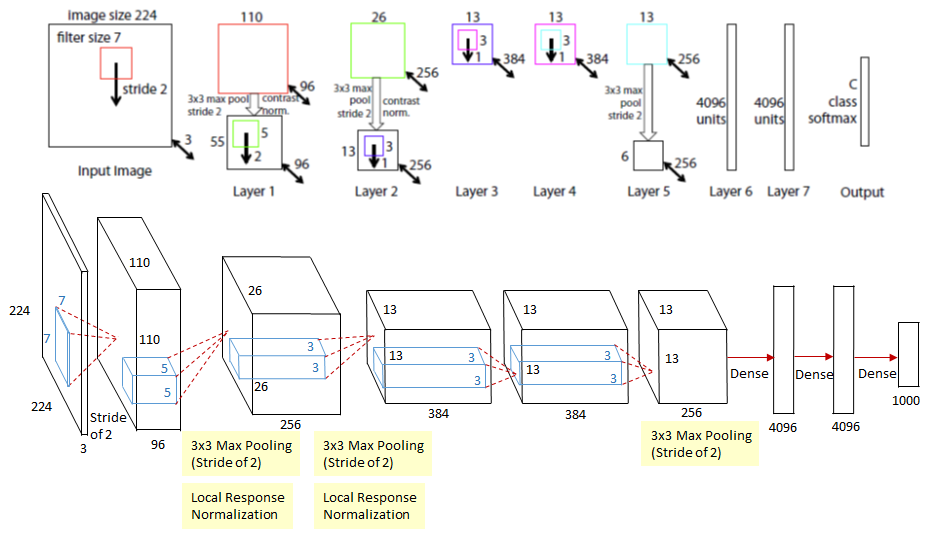
\includegraphics[width=0.7\linewidth]{img/02-04} \end{center}

\hspace{0pt}如图所示,ZFNet与AlexNet类似,都是由8层网络组成的卷积神经网络,其中包含5层卷积层和3层全连接层。两个网络结构最大的不同在于,ZFNet第一层卷积采用了\(7\times7\times3/2\)的卷积核替代了AlexNet中第一层卷积核\(11\times11\times3/4\)的卷积核。ZFNet相比于AlexNet在第一层输出的特征图中包含更多中间频率的信息,而AlexNet第一层输出的特征图大多是低频或高频的信息,对中间频率特征的缺失导致后续网络层次能够学习到的特征不够细致,而导致这个问题的根本原因在于AlexNet在第一层中采用的卷积核和步长过大。

\begin{center}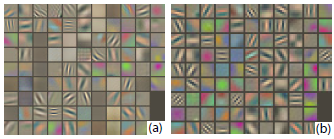
\includegraphics[width=0.7\linewidth]{img/02-05} \end{center}

\begin{center}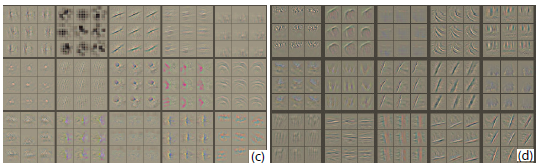
\includegraphics[width=0.7\linewidth]{img/02-06} \end{center}

(a)ZFNet第一层输出的特征图(b)AlexNet第一层输出的特征图(c)AlexNet第二层输出的特征图(d)ZFNet第二层输出的特征图

\begin{longtable}[]{@{}ccccc@{}}
\toprule
\begin{minipage}[b]{0.17\columnwidth}\centering
网络层\strut
\end{minipage} & \begin{minipage}[b]{0.17\columnwidth}\centering
输入尺寸\strut
\end{minipage} & \begin{minipage}[b]{0.17\columnwidth}\centering
核尺寸\strut
\end{minipage} & \begin{minipage}[b]{0.17\columnwidth}\centering
输出尺寸\strut
\end{minipage} & \begin{minipage}[b]{0.17\columnwidth}\centering
可训练参数量\strut
\end{minipage}\tabularnewline
\midrule
\endhead
\begin{minipage}[t]{0.17\columnwidth}\centering
卷积层\(C_1\) \(^*\)\strut
\end{minipage} & \begin{minipage}[t]{0.17\columnwidth}\centering
\(224\times224\times3\)\strut
\end{minipage} & \begin{minipage}[t]{0.17\columnwidth}\centering
\(7\times7\times3/2,96\)\strut
\end{minipage} & \begin{minipage}[t]{0.17\columnwidth}\centering
\(110\times110\times96\)\strut
\end{minipage} & \begin{minipage}[t]{0.17\columnwidth}\centering
\((7\times7\times3+1)\times96\)\strut
\end{minipage}\tabularnewline
\begin{minipage}[t]{0.17\columnwidth}\centering
下采样层\(S_{max}\)\strut
\end{minipage} & \begin{minipage}[t]{0.17\columnwidth}\centering
\(110\times110\times96\)\strut
\end{minipage} & \begin{minipage}[t]{0.17\columnwidth}\centering
\(3\times3/2\)\strut
\end{minipage} & \begin{minipage}[t]{0.17\columnwidth}\centering
\(55\times55\times96\)\strut
\end{minipage} & \begin{minipage}[t]{0.17\columnwidth}\centering
0\strut
\end{minipage}\tabularnewline
\begin{minipage}[t]{0.17\columnwidth}\centering
卷积层\(C_2\) \(^*\)\strut
\end{minipage} & \begin{minipage}[t]{0.17\columnwidth}\centering
\(55\times55\times96\)\strut
\end{minipage} & \begin{minipage}[t]{0.17\columnwidth}\centering
\(5\times5\times96/2,256\)\strut
\end{minipage} & \begin{minipage}[t]{0.17\columnwidth}\centering
\(26\times26\times256\)\strut
\end{minipage} & \begin{minipage}[t]{0.17\columnwidth}\centering
\((5\times5\times96+1)\times256\)\strut
\end{minipage}\tabularnewline
\begin{minipage}[t]{0.17\columnwidth}\centering
下采样层\(S_{max}\)\strut
\end{minipage} & \begin{minipage}[t]{0.17\columnwidth}\centering
\(26\times26\times256\)\strut
\end{minipage} & \begin{minipage}[t]{0.17\columnwidth}\centering
\(3\times3/2\)\strut
\end{minipage} & \begin{minipage}[t]{0.17\columnwidth}\centering
\(13\times13\times256\)\strut
\end{minipage} & \begin{minipage}[t]{0.17\columnwidth}\centering
0\strut
\end{minipage}\tabularnewline
\begin{minipage}[t]{0.17\columnwidth}\centering
卷积层\(C_3\)\strut
\end{minipage} & \begin{minipage}[t]{0.17\columnwidth}\centering
\(13\times13\times256\)\strut
\end{minipage} & \begin{minipage}[t]{0.17\columnwidth}\centering
\(3\times3\times256/1,384\)\strut
\end{minipage} & \begin{minipage}[t]{0.17\columnwidth}\centering
\(13\times13\times384\)\strut
\end{minipage} & \begin{minipage}[t]{0.17\columnwidth}\centering
\((3\times3\times256+1)\times384\)\strut
\end{minipage}\tabularnewline
\begin{minipage}[t]{0.17\columnwidth}\centering
卷积层\(C_4\)\strut
\end{minipage} & \begin{minipage}[t]{0.17\columnwidth}\centering
\(13\times13\times384\)\strut
\end{minipage} & \begin{minipage}[t]{0.17\columnwidth}\centering
\(3\times3\times384/1,384\)\strut
\end{minipage} & \begin{minipage}[t]{0.17\columnwidth}\centering
\(13\times13\times384\)\strut
\end{minipage} & \begin{minipage}[t]{0.17\columnwidth}\centering
\((3\times3\times384+1)\times384\)\strut
\end{minipage}\tabularnewline
\begin{minipage}[t]{0.17\columnwidth}\centering
卷积层\(C_5\)\strut
\end{minipage} & \begin{minipage}[t]{0.17\columnwidth}\centering
\(13\times13\times384\)\strut
\end{minipage} & \begin{minipage}[t]{0.17\columnwidth}\centering
\(3\times3\times384/1,256\)\strut
\end{minipage} & \begin{minipage}[t]{0.17\columnwidth}\centering
\(13\times13\times256\)\strut
\end{minipage} & \begin{minipage}[t]{0.17\columnwidth}\centering
\((3\times3\times384+1)\times256\)\strut
\end{minipage}\tabularnewline
\begin{minipage}[t]{0.17\columnwidth}\centering
下采样层\(S_{max}\)\strut
\end{minipage} & \begin{minipage}[t]{0.17\columnwidth}\centering
\(13\times13\times256\)\strut
\end{minipage} & \begin{minipage}[t]{0.17\columnwidth}\centering
\(3\times3/2\)\strut
\end{minipage} & \begin{minipage}[t]{0.17\columnwidth}\centering
\(6\times6\times256\)\strut
\end{minipage} & \begin{minipage}[t]{0.17\columnwidth}\centering
0\strut
\end{minipage}\tabularnewline
\begin{minipage}[t]{0.17\columnwidth}\centering
全连接层\(F_6\)\strut
\end{minipage} & \begin{minipage}[t]{0.17\columnwidth}\centering
\(6\times6\times256\)\strut
\end{minipage} & \begin{minipage}[t]{0.17\columnwidth}\centering
\(9216\times4096\)\strut
\end{minipage} & \begin{minipage}[t]{0.17\columnwidth}\centering
\(1\times1\times4096\)\strut
\end{minipage} & \begin{minipage}[t]{0.17\columnwidth}\centering
\((9216+1)\times4096\)\strut
\end{minipage}\tabularnewline
\begin{minipage}[t]{0.17\columnwidth}\centering
全连接层\(F_7\)\strut
\end{minipage} & \begin{minipage}[t]{0.17\columnwidth}\centering
\(1\times1\times4096\)\strut
\end{minipage} & \begin{minipage}[t]{0.17\columnwidth}\centering
\(4096\times4096\)\strut
\end{minipage} & \begin{minipage}[t]{0.17\columnwidth}\centering
\(1\times1\times4096\)\strut
\end{minipage} & \begin{minipage}[t]{0.17\columnwidth}\centering
\((4096+1)\times4096\)\strut
\end{minipage}\tabularnewline
\begin{minipage}[t]{0.17\columnwidth}\centering
全连接层\(F_8\)\strut
\end{minipage} & \begin{minipage}[t]{0.17\columnwidth}\centering
\(1\times1\times4096\)\strut
\end{minipage} & \begin{minipage}[t]{0.17\columnwidth}\centering
\(4096\times1000\)\strut
\end{minipage} & \begin{minipage}[t]{0.17\columnwidth}\centering
\(1\times1\times1000\)\strut
\end{minipage} & \begin{minipage}[t]{0.17\columnwidth}\centering
\((4096+1)\times1000\)\strut
\end{minipage}\tabularnewline
\bottomrule
\end{longtable}

\begin{itemize}
\item
  卷积层\(C_1\)与AlexNet中的\(C_1\)有所不同,采用\(7\times7\times3/2\)的卷积核代替\(11\times11\times3/4​\),使第一层卷积输出的结果可以包含更多的中频率特征,对后续网络层中多样化的特征组合提供更多选择,有利于捕捉更细致的特征。
\item
  卷积层\(C_2\)采用了步长2的卷积核,区别于AlexNet中\(C_2\)的卷积核步长,所以输出的维度有所差异。
\end{itemize}

\hypertarget{ux6a21ux578bux7279ux6027-2}{%
\subsection{模型特性}\label{ux6a21ux578bux7279ux6027-2}}

\hspace{0pt}ZFNet与AlexNet在结构上几乎相同,此部分虽属于模型特性,但准确地说应该是ZFNet原论文中可视化技术的贡献。

\begin{itemize}
\tightlist
\item
  可视化技术揭露了激发模型中每层单独的特征图。
\item
  可视化技术允许观察在训练阶段特征的演变过程且诊断出模型的潜在问题。
\item
  可视化技术用到了多层解卷积网络,即由特征激活返回到输入像素空间。
\item
  可视化技术进行了分类器输出的敏感性分析,即通过阻止部分输入图像来揭示那部分对于分类是重要的。
\item
  可视化技术提供了一个非参数的不变性来展示来自训练集的哪一块激活哪个特征图,不仅需要裁剪输入图片,而且自上而下的投影来揭露来自每块的结构激活一个特征图。
\item
  可视化技术依赖于解卷积操作,即卷积操作的逆过程,将特征映射到像素上。
\end{itemize}

\hypertarget{network-in-network}{%
\section{Network in Network}\label{network-in-network}}

\hypertarget{ux6a21ux578bux4ecbux7ecd-3}{%
\subsection{模型介绍}\label{ux6a21ux578bux4ecbux7ecd-3}}

Network In Network (NIN)是由\(Min Lin\)等人提出,在CIFAR-10和CIFAR-100分类任务中达到当时的最好水平,因其网络结构是由三个多层感知机堆叠而被成为NIN\(^{[5]}\)。NIN以一种全新的角度审视了卷积神经网络中的卷积核设计,通过引入子网络结构代替纯卷积中的线性映射部分,这种形式的网络结构激发了更复杂的卷积神经网络的结构设计,其中下一节中介绍的GoogLeNet的Inception结构就是来源于这个思想。

\hypertarget{ux6a21ux578bux7ed3ux6784-3}{%
\subsection{模型结构}\label{ux6a21ux578bux7ed3ux6784-3}}

\begin{center}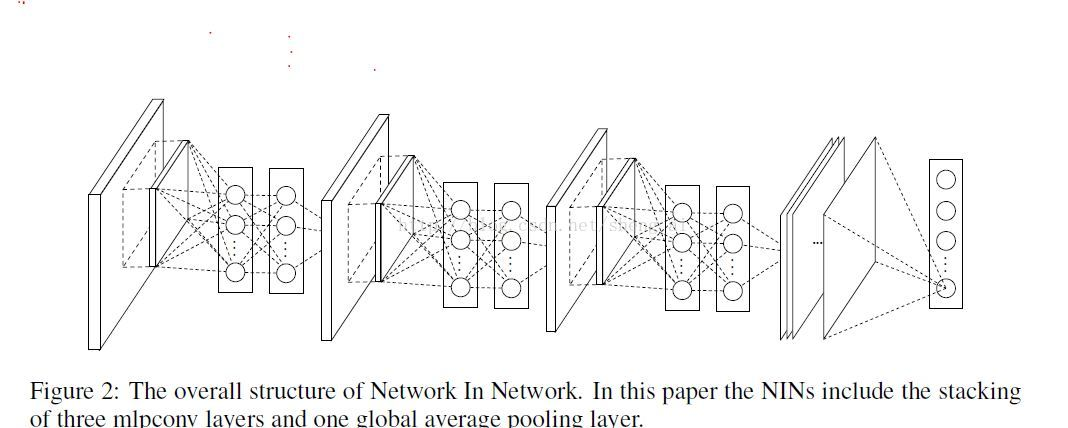
\includegraphics[width=0.7\linewidth]{img/02-07} \end{center}

\hspace{0pt}NIN由三层的多层感知卷积层(MLPConv Layer)构成,每一层多层感知卷积层内部由若干层的局部全连接层和非线性激活函数组成,代替了传统卷积层中采用的线性卷积核。在网络推理(inference)时,这个多层感知器会对输入特征图的局部特征进行划窗计算,并且每个划窗的局部特征图对应的乘积的权重是共享的,这两点是和传统卷积操作完全一致的,最大的不同在于多层感知器对局部特征进行了非线性的映射,而传统卷积的方式是线性的。NIN的网络参数配置表4.4所示(原论文并未给出网络参数,表中参数为编者结合网络结构图和CIFAR-100数据集以\(3\times3\)卷积为例给出)。

\begin{longtable}[]{@{}ccccc@{}}
\toprule
\begin{minipage}[b]{0.16\columnwidth}\centering
网络层\strut
\end{minipage} & \begin{minipage}[b]{0.18\columnwidth}\centering
输入尺寸\strut
\end{minipage} & \begin{minipage}[b]{0.16\columnwidth}\centering
核尺寸\strut
\end{minipage} & \begin{minipage}[b]{0.20\columnwidth}\centering
输出尺寸\strut
\end{minipage} & \begin{minipage}[b]{0.18\columnwidth}\centering
参数个数\strut
\end{minipage}\tabularnewline
\midrule
\endhead
\begin{minipage}[t]{0.16\columnwidth}\centering
局部全连接层\(L_{11}\) \(^*\)\strut
\end{minipage} & \begin{minipage}[t]{0.18\columnwidth}\centering
\(32\times32\times3\)\strut
\end{minipage} & \begin{minipage}[t]{0.16\columnwidth}\centering
\((3\times3)\times16/1\)\strut
\end{minipage} & \begin{minipage}[t]{0.20\columnwidth}\centering
\(30\times30\times16\)\strut
\end{minipage} & \begin{minipage}[t]{0.18\columnwidth}\centering
\((3\times3\times3+1)\times16\)\strut
\end{minipage}\tabularnewline
\begin{minipage}[t]{0.16\columnwidth}\centering
全连接层\(L_{12}\) \(^*\)\strut
\end{minipage} & \begin{minipage}[t]{0.18\columnwidth}\centering
\(30\times30\times16\)\strut
\end{minipage} & \begin{minipage}[t]{0.16\columnwidth}\centering
\(16\times16\)\strut
\end{minipage} & \begin{minipage}[t]{0.20\columnwidth}\centering
\(30\times30\times16\)\strut
\end{minipage} & \begin{minipage}[t]{0.18\columnwidth}\centering
\(((16+1)\times16)\)\strut
\end{minipage}\tabularnewline
\begin{minipage}[t]{0.16\columnwidth}\centering
局部全连接层\(L_{21}\)\strut
\end{minipage} & \begin{minipage}[t]{0.18\columnwidth}\centering
\(30\times30\times16\)\strut
\end{minipage} & \begin{minipage}[t]{0.16\columnwidth}\centering
\((3\times3)\times64/1\)\strut
\end{minipage} & \begin{minipage}[t]{0.20\columnwidth}\centering
\(28\times28\times64\)\strut
\end{minipage} & \begin{minipage}[t]{0.18\columnwidth}\centering
\((3\times3\times16+1)\times64\)\strut
\end{minipage}\tabularnewline
\begin{minipage}[t]{0.16\columnwidth}\centering
全连接层\(L_{22}\)\strut
\end{minipage} & \begin{minipage}[t]{0.18\columnwidth}\centering
\(28\times28\times64\)\strut
\end{minipage} & \begin{minipage}[t]{0.16\columnwidth}\centering
\(64\times64\)\strut
\end{minipage} & \begin{minipage}[t]{0.20\columnwidth}\centering
\(28\times28\times64\)\strut
\end{minipage} & \begin{minipage}[t]{0.18\columnwidth}\centering
\(((64+1)\times64)\)\strut
\end{minipage}\tabularnewline
\begin{minipage}[t]{0.16\columnwidth}\centering
局部全连接层\(L_{31}\)\strut
\end{minipage} & \begin{minipage}[t]{0.18\columnwidth}\centering
\(28\times28\times64\)\strut
\end{minipage} & \begin{minipage}[t]{0.16\columnwidth}\centering
\((3\times3)\times100/1\)\strut
\end{minipage} & \begin{minipage}[t]{0.20\columnwidth}\centering
\(26\times26\times100\)\strut
\end{minipage} & \begin{minipage}[t]{0.18\columnwidth}\centering
\((3\times3\times64+1)\times100\)\strut
\end{minipage}\tabularnewline
\begin{minipage}[t]{0.16\columnwidth}\centering
全连接层\(L_{32}\)\strut
\end{minipage} & \begin{minipage}[t]{0.18\columnwidth}\centering
\(26\times26\times100\)\strut
\end{minipage} & \begin{minipage}[t]{0.16\columnwidth}\centering
\(100\times100\)\strut
\end{minipage} & \begin{minipage}[t]{0.20\columnwidth}\centering
\(26\times26\times100\)\strut
\end{minipage} & \begin{minipage}[t]{0.18\columnwidth}\centering
\(((100+1)\times100)\)\strut
\end{minipage}\tabularnewline
\begin{minipage}[t]{0.16\columnwidth}\centering
全局平均采样\(GAP\) \(^*\)\strut
\end{minipage} & \begin{minipage}[t]{0.18\columnwidth}\centering
\(26\times26\times100\)\strut
\end{minipage} & \begin{minipage}[t]{0.16\columnwidth}\centering
\(26\times26\times100/1\)\strut
\end{minipage} & \begin{minipage}[t]{0.20\columnwidth}\centering
\(1\times1\times100\)\strut
\end{minipage} & \begin{minipage}[t]{0.18\columnwidth}\centering
\(0\)\strut
\end{minipage}\tabularnewline
\bottomrule
\end{longtable}

\begin{itemize}
\item
  局部全连接层\(L_{11}\)实际上是对原始输入图像进行划窗式的全连接操作,因此划窗得到的输出特征尺寸为\(30\times30\)(\(\frac{32-3_k+1}{1_{stride}}=30\))
\item
  全连接层\(L_{12}\)是紧跟\(L_{11}\)后的全连接操作,输入的特征是划窗后经过激活的局部响应特征,因此仅需连接\(L_{11}\)和\(L_{12}\)的节点即可,而每个局部全连接层和紧接的全连接层构成代替卷积操作的多层感知卷积层(MLPConv)。
\item
  全局平均采样层或全局平均池化层\(GAP\)(Global Average Pooling)将\(L_{32}\)输出的每一个特征图进行全局的平均池化操作,直接得到最后的类别数,可以有效地减少参数量。
\end{itemize}

\hypertarget{ux6a21ux578bux7279ux70b9}{%
\subsection{模型特点}\label{ux6a21ux578bux7279ux70b9}}

\begin{itemize}
\item
  使用多层感知机结构来代替卷积的滤波操作,不但有效减少卷积核数过多而导致的参数量暴涨问题,还能通过引入非线性的映射来提高模型对特征的抽象能力。
\item
  使用全局平均池化来代替最后一个全连接层,能够有效地减少参数量(没有可训练参数),同时池化用到了整个特征图的信息,对空间信息的转换更加鲁棒,最后得到的输出结果可直接作为对应类别的置信度。
\end{itemize}

\hypertarget{vggnet}{%
\section{VGGNet}\label{vggnet}}

\hypertarget{ux6a21ux578bux4ecbux7ecd-4}{%
\subsection{模型介绍}\label{ux6a21ux578bux4ecbux7ecd-4}}

\hspace{0pt}VGGNet是由牛津大学视觉几何小组(Visual Geometry Group, VGG)提出的一种深层卷积网络结构,他们以7.32\%的错误率赢得了2014年ILSVRC分类任务的亚军(冠军由GoogLeNet以6.65\%的错误率夺得)和25.32\%的错误率夺得定位任务(Localization)的第一名(GoogLeNet错误率为26.44\%)\(^{[5]}\),网络名称VGGNet取自该小组名缩写。VGGNet是首批把图像分类的错误率降低到10\%以内模型,同时该网络所采用的\(3\times3\)卷积核的思想是后来许多模型的基础,该模型发表在2015年国际学习表征会议(International Conference On Learning Representations, ICLR)后至今被引用的次数已经超过1万4千余次。

\hypertarget{ux6a21ux578bux7ed3ux6784-4}{%
\subsection{模型结构}\label{ux6a21ux578bux7ed3ux6784-4}}

\begin{center}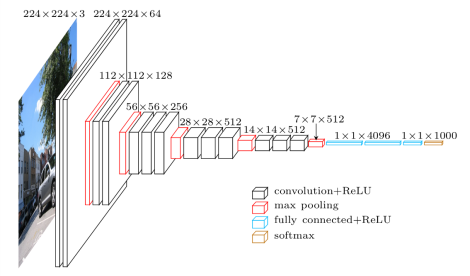
\includegraphics[width=0.7\linewidth]{img/02-08} \end{center}

\hspace{0pt}在原论文中的VGGNet包含了6个版本的演进,分别对应VGG11、VGG11-LRN、VGG13、VGG16-1、VGG16-3和VGG19,不同的后缀数值表示不同的网络层数(VGG11-LRN表示在第一层中采用了LRN的VGG11,VGG16-1表示后三组卷积块中最后一层卷积采用卷积核尺寸为\(1\times1\),相应的VGG16-3表示卷积核尺寸为\(3\times3\)),本节介绍的VGG16为VGG16-3。上图中的VGG16体现了VGGNet的核心思路,使用\(3\times3\)的卷积组合代替大尺寸的卷积(2个\(3\times3卷积即可与\)\(5\times5\)卷积拥有相同的感受视野),网络参数设置如下表所示。

\begin{longtable}[]{@{}ccccc@{}}
\toprule
\begin{minipage}[b]{0.17\columnwidth}\centering
网络层\strut
\end{minipage} & \begin{minipage}[b]{0.17\columnwidth}\centering
输入尺寸\strut
\end{minipage} & \begin{minipage}[b]{0.17\columnwidth}\centering
核尺寸\strut
\end{minipage} & \begin{minipage}[b]{0.17\columnwidth}\centering
输出尺寸\strut
\end{minipage} & \begin{minipage}[b]{0.17\columnwidth}\centering
参数个数\strut
\end{minipage}\tabularnewline
\midrule
\endhead
\begin{minipage}[t]{0.17\columnwidth}\centering
卷积层\(C_{11}\)\strut
\end{minipage} & \begin{minipage}[t]{0.17\columnwidth}\centering
\(224\times224\times3\)\strut
\end{minipage} & \begin{minipage}[t]{0.17\columnwidth}\centering
\(3\times3\times64/1\)\strut
\end{minipage} & \begin{minipage}[t]{0.17\columnwidth}\centering
\(224\times224\times64\)\strut
\end{minipage} & \begin{minipage}[t]{0.17\columnwidth}\centering
\((3\times3\times3+1)\times64\)\strut
\end{minipage}\tabularnewline
\begin{minipage}[t]{0.17\columnwidth}\centering
卷积层\(C_{12}\)\strut
\end{minipage} & \begin{minipage}[t]{0.17\columnwidth}\centering
\(224\times224\times64\)\strut
\end{minipage} & \begin{minipage}[t]{0.17\columnwidth}\centering
\(3\times3\times64/1\)\strut
\end{minipage} & \begin{minipage}[t]{0.17\columnwidth}\centering
\(224\times224\times64\)\strut
\end{minipage} & \begin{minipage}[t]{0.17\columnwidth}\centering
\((3\times3\times64+1)\times64\)\strut
\end{minipage}\tabularnewline
\begin{minipage}[t]{0.17\columnwidth}\centering
下采样层\(S_{max1}\)\strut
\end{minipage} & \begin{minipage}[t]{0.17\columnwidth}\centering
\(224\times224\times64\)\strut
\end{minipage} & \begin{minipage}[t]{0.17\columnwidth}\centering
\(2\times2/2\)\strut
\end{minipage} & \begin{minipage}[t]{0.17\columnwidth}\centering
\(112\times112\times64\)\strut
\end{minipage} & \begin{minipage}[t]{0.17\columnwidth}\centering
\(0\)\strut
\end{minipage}\tabularnewline
\begin{minipage}[t]{0.17\columnwidth}\centering
卷积层\(C_{21}\)\strut
\end{minipage} & \begin{minipage}[t]{0.17\columnwidth}\centering
\(112\times112\times64\)\strut
\end{minipage} & \begin{minipage}[t]{0.17\columnwidth}\centering
\(3\times3\times128/1\)\strut
\end{minipage} & \begin{minipage}[t]{0.17\columnwidth}\centering
\(112\times112\times128\)\strut
\end{minipage} & \begin{minipage}[t]{0.17\columnwidth}\centering
\((3\times3\times64+1)\times128\)\strut
\end{minipage}\tabularnewline
\begin{minipage}[t]{0.17\columnwidth}\centering
卷积层\(C_{22}\)\strut
\end{minipage} & \begin{minipage}[t]{0.17\columnwidth}\centering
\(112\times112\times128\)\strut
\end{minipage} & \begin{minipage}[t]{0.17\columnwidth}\centering
\(3\times3\times128/1\)\strut
\end{minipage} & \begin{minipage}[t]{0.17\columnwidth}\centering
\(112\times112\times128\)\strut
\end{minipage} & \begin{minipage}[t]{0.17\columnwidth}\centering
\((3\times3\times128+1)\times128\)\strut
\end{minipage}\tabularnewline
\begin{minipage}[t]{0.17\columnwidth}\centering
下采样层\(S_{max2}\)\strut
\end{minipage} & \begin{minipage}[t]{0.17\columnwidth}\centering
\(112\times112\times128\)\strut
\end{minipage} & \begin{minipage}[t]{0.17\columnwidth}\centering
\(2\times2/2\)\strut
\end{minipage} & \begin{minipage}[t]{0.17\columnwidth}\centering
\(56\times56\times128\)\strut
\end{minipage} & \begin{minipage}[t]{0.17\columnwidth}\centering
\(0\)\strut
\end{minipage}\tabularnewline
\begin{minipage}[t]{0.17\columnwidth}\centering
卷积层\(C_{31}\)\strut
\end{minipage} & \begin{minipage}[t]{0.17\columnwidth}\centering
\(56\times56\times128\)\strut
\end{minipage} & \begin{minipage}[t]{0.17\columnwidth}\centering
\(3\times3\times256/1\)\strut
\end{minipage} & \begin{minipage}[t]{0.17\columnwidth}\centering
\(56\times56\times256\)\strut
\end{minipage} & \begin{minipage}[t]{0.17\columnwidth}\centering
\((3\times3\times128+1)\times256\)\strut
\end{minipage}\tabularnewline
\begin{minipage}[t]{0.17\columnwidth}\centering
卷积层\(C_{32}\)\strut
\end{minipage} & \begin{minipage}[t]{0.17\columnwidth}\centering
\(56\times56\times256\)\strut
\end{minipage} & \begin{minipage}[t]{0.17\columnwidth}\centering
\(3\times3\times256/1\)\strut
\end{minipage} & \begin{minipage}[t]{0.17\columnwidth}\centering
\(56\times56\times256\)\strut
\end{minipage} & \begin{minipage}[t]{0.17\columnwidth}\centering
\((3\times3\times256+1)\times256\)\strut
\end{minipage}\tabularnewline
\begin{minipage}[t]{0.17\columnwidth}\centering
卷积层\(C_{33}\)\strut
\end{minipage} & \begin{minipage}[t]{0.17\columnwidth}\centering
\(56\times56\times256\)\strut
\end{minipage} & \begin{minipage}[t]{0.17\columnwidth}\centering
\(26\times26\times256/1\)\strut
\end{minipage} & \begin{minipage}[t]{0.17\columnwidth}\centering
\(56\times56\times256\)\strut
\end{minipage} & \begin{minipage}[t]{0.17\columnwidth}\centering
\((3\times3\times256+1)\times256\)\strut
\end{minipage}\tabularnewline
\begin{minipage}[t]{0.17\columnwidth}\centering
下采样层\(S_{max3}\)\strut
\end{minipage} & \begin{minipage}[t]{0.17\columnwidth}\centering
\(56\times56\times256\)\strut
\end{minipage} & \begin{minipage}[t]{0.17\columnwidth}\centering
\(2\times2/2\)\strut
\end{minipage} & \begin{minipage}[t]{0.17\columnwidth}\centering
\(28\times28\times256\)\strut
\end{minipage} & \begin{minipage}[t]{0.17\columnwidth}\centering
\(0\)\strut
\end{minipage}\tabularnewline
\begin{minipage}[t]{0.17\columnwidth}\centering
卷积层\(C_{41}\)\strut
\end{minipage} & \begin{minipage}[t]{0.17\columnwidth}\centering
\(28\times28\times256\)\strut
\end{minipage} & \begin{minipage}[t]{0.17\columnwidth}\centering
\(3\times3\times512/1\)\strut
\end{minipage} & \begin{minipage}[t]{0.17\columnwidth}\centering
\(28\times28\times512\)\strut
\end{minipage} & \begin{minipage}[t]{0.17\columnwidth}\centering
\((3\times3\times256+1)\times512\)\strut
\end{minipage}\tabularnewline
\begin{minipage}[t]{0.17\columnwidth}\centering
卷积层\(C_{42}\)\strut
\end{minipage} & \begin{minipage}[t]{0.17\columnwidth}\centering
\(28\times28\times512\)\strut
\end{minipage} & \begin{minipage}[t]{0.17\columnwidth}\centering
\(3\times3\times512/1\)\strut
\end{minipage} & \begin{minipage}[t]{0.17\columnwidth}\centering
\(28\times28\times512\)\strut
\end{minipage} & \begin{minipage}[t]{0.17\columnwidth}\centering
\((3\times3\times512+1)\times512\)\strut
\end{minipage}\tabularnewline
\begin{minipage}[t]{0.17\columnwidth}\centering
卷积层\(C_{43}\)\strut
\end{minipage} & \begin{minipage}[t]{0.17\columnwidth}\centering
\(28\times28\times512\)\strut
\end{minipage} & \begin{minipage}[t]{0.17\columnwidth}\centering
\(3\times3\times512/1\)\strut
\end{minipage} & \begin{minipage}[t]{0.17\columnwidth}\centering
\(28\times28\times512\)\strut
\end{minipage} & \begin{minipage}[t]{0.17\columnwidth}\centering
\((3\times3\times512+1)\times512\)\strut
\end{minipage}\tabularnewline
\begin{minipage}[t]{0.17\columnwidth}\centering
下采样层\(S_{max4}\)\strut
\end{minipage} & \begin{minipage}[t]{0.17\columnwidth}\centering
\(28\times28\times512\)\strut
\end{minipage} & \begin{minipage}[t]{0.17\columnwidth}\centering
\(2\times2/2\)\strut
\end{minipage} & \begin{minipage}[t]{0.17\columnwidth}\centering
\(14\times14\times512\)\strut
\end{minipage} & \begin{minipage}[t]{0.17\columnwidth}\centering
\(0\)\strut
\end{minipage}\tabularnewline
\begin{minipage}[t]{0.17\columnwidth}\centering
卷积层\(C_{51}\)\strut
\end{minipage} & \begin{minipage}[t]{0.17\columnwidth}\centering
\(14\times14\times512\)\strut
\end{minipage} & \begin{minipage}[t]{0.17\columnwidth}\centering
\(3\times3\times512/1\)\strut
\end{minipage} & \begin{minipage}[t]{0.17\columnwidth}\centering
\(14\times14\times512\)\strut
\end{minipage} & \begin{minipage}[t]{0.17\columnwidth}\centering
\((3\times3\times512+1)\times512\)\strut
\end{minipage}\tabularnewline
\begin{minipage}[t]{0.17\columnwidth}\centering
卷积层\(C_{52}\)\strut
\end{minipage} & \begin{minipage}[t]{0.17\columnwidth}\centering
\(14\times14\times512\)\strut
\end{minipage} & \begin{minipage}[t]{0.17\columnwidth}\centering
\(3\times3\times512/1\)\strut
\end{minipage} & \begin{minipage}[t]{0.17\columnwidth}\centering
\(14\times14\times512\)\strut
\end{minipage} & \begin{minipage}[t]{0.17\columnwidth}\centering
\((3\times3\times512+1)\times512\)\strut
\end{minipage}\tabularnewline
\begin{minipage}[t]{0.17\columnwidth}\centering
卷积层\(C_{53}\)\strut
\end{minipage} & \begin{minipage}[t]{0.17\columnwidth}\centering
\(14\times14\times512\)\strut
\end{minipage} & \begin{minipage}[t]{0.17\columnwidth}\centering
\(3\times3\times512/1\)\strut
\end{minipage} & \begin{minipage}[t]{0.17\columnwidth}\centering
\(14\times14\times512\)\strut
\end{minipage} & \begin{minipage}[t]{0.17\columnwidth}\centering
\((3\times3\times512+1)\times512\)\strut
\end{minipage}\tabularnewline
\begin{minipage}[t]{0.17\columnwidth}\centering
下采样层\(S_{max5}\)\strut
\end{minipage} & \begin{minipage}[t]{0.17\columnwidth}\centering
\(14\times14\times512\)\strut
\end{minipage} & \begin{minipage}[t]{0.17\columnwidth}\centering
\(2\times2/2\)\strut
\end{minipage} & \begin{minipage}[t]{0.17\columnwidth}\centering
\(7\times7\times512\)\strut
\end{minipage} & \begin{minipage}[t]{0.17\columnwidth}\centering
\(0\)\strut
\end{minipage}\tabularnewline
\begin{minipage}[t]{0.17\columnwidth}\centering
全连接层\(FC_{1}\)\strut
\end{minipage} & \begin{minipage}[t]{0.17\columnwidth}\centering
\(7\times7\times512\)\strut
\end{minipage} & \begin{minipage}[t]{0.17\columnwidth}\centering
\((7\times7\times512)\times4096\)\strut
\end{minipage} & \begin{minipage}[t]{0.17\columnwidth}\centering
\(1\times4096\)\strut
\end{minipage} & \begin{minipage}[t]{0.17\columnwidth}\centering
\((7\times7\times512+1)\times4096\)\strut
\end{minipage}\tabularnewline
\begin{minipage}[t]{0.17\columnwidth}\centering
全连接层\(FC_{2}\)\strut
\end{minipage} & \begin{minipage}[t]{0.17\columnwidth}\centering
\(1\times4096\)\strut
\end{minipage} & \begin{minipage}[t]{0.17\columnwidth}\centering
\(4096\times4096\)\strut
\end{minipage} & \begin{minipage}[t]{0.17\columnwidth}\centering
\(1\times4096\)\strut
\end{minipage} & \begin{minipage}[t]{0.17\columnwidth}\centering
\((4096+1)\times4096\)\strut
\end{minipage}\tabularnewline
\begin{minipage}[t]{0.17\columnwidth}\centering
全连接层\(FC_{3}\)\strut
\end{minipage} & \begin{minipage}[t]{0.17\columnwidth}\centering
\(1\times4096\)\strut
\end{minipage} & \begin{minipage}[t]{0.17\columnwidth}\centering
\(4096\times1000\)\strut
\end{minipage} & \begin{minipage}[t]{0.17\columnwidth}\centering
\(1\times1000\)\strut
\end{minipage} & \begin{minipage}[t]{0.17\columnwidth}\centering
\((4096+1)\times1000\)\strut
\end{minipage}\tabularnewline
\bottomrule
\end{longtable}

\hypertarget{ux6a21ux578bux7279ux6027-3}{%
\subsection{模型特性}\label{ux6a21ux578bux7279ux6027-3}}

\begin{itemize}
\tightlist
\item
  整个网络都使用了同样大小的卷积核尺寸\(3\times3\)和最大池化尺寸\(2\times2\)。
\item
  \(1\times1\)卷积的意义主要在于线性变换,而输入通道数和输出通道数不变,没有发生降维。
\item
  两个\(3\times3\)的卷积层串联相当于1个\(5\times5\)的卷积层,感受野大小为\(5\times5\)。同样地,3个\(3\times3\)的卷积层串联的效果则相当于1个\(7\times7\)的卷积层。这样的连接方式使得网络参数量更小,而且多层的激活函数令网络对特征的学习能力更强。
\item
  VGGNet在训练时有一个小技巧,先训练浅层的的简单网络VGG11,再复用VGG11的权重来初始化VGG13,如此反复训练并初始化VGG19,能够使训练时收敛的速度更快。
\item
  在训练过程中使用多尺度的变换对原始数据做数据增强,使得模型不易过拟合。
\end{itemize}

\hypertarget{googlenet}{%
\section{GoogLeNet}\label{googlenet}}

\hypertarget{ux6a21ux578bux4ecbux7ecd-5}{%
\subsection{模型介绍}\label{ux6a21ux578bux4ecbux7ecd-5}}

GoogLeNet作为2014年ILSVRC在分类任务上的冠军,以6.65\%的错误率力压VGGNet等模型,在分类的准确率上面相比过去两届冠军ZFNet和AlexNet都有很大的提升。从名字\textbf{GoogLe}Net可以知道这是来自谷歌工程师所设计的网络结构,而名字中Goog\textbf{LeNet}更是致敬了LeNet\(^{[0]}\)。GoogLeNet中最核心的部分是其内部子网络结构Inception,该结构灵感来源于NIN,至今已经经历了四次版本迭代(Inception\(_{v1-4}\))。

\begin{center}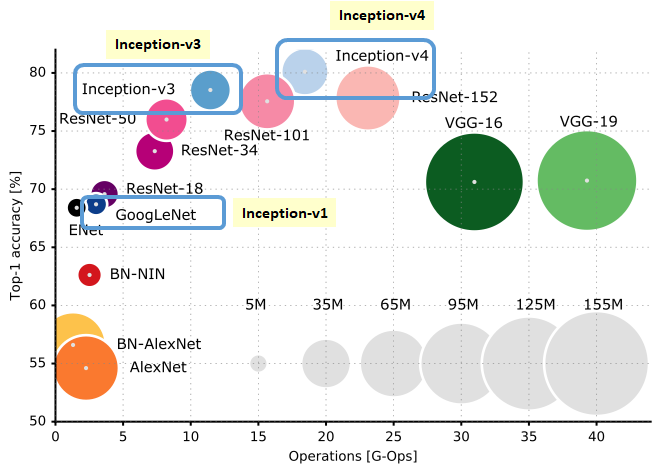
\includegraphics[width=0.7\linewidth]{img/02-09} \end{center}

\hypertarget{ux6a21ux578bux7ed3ux6784-5}{%
\subsection{4.6.2 模型结构}\label{ux6a21ux578bux7ed3ux6784-5}}

\begin{center}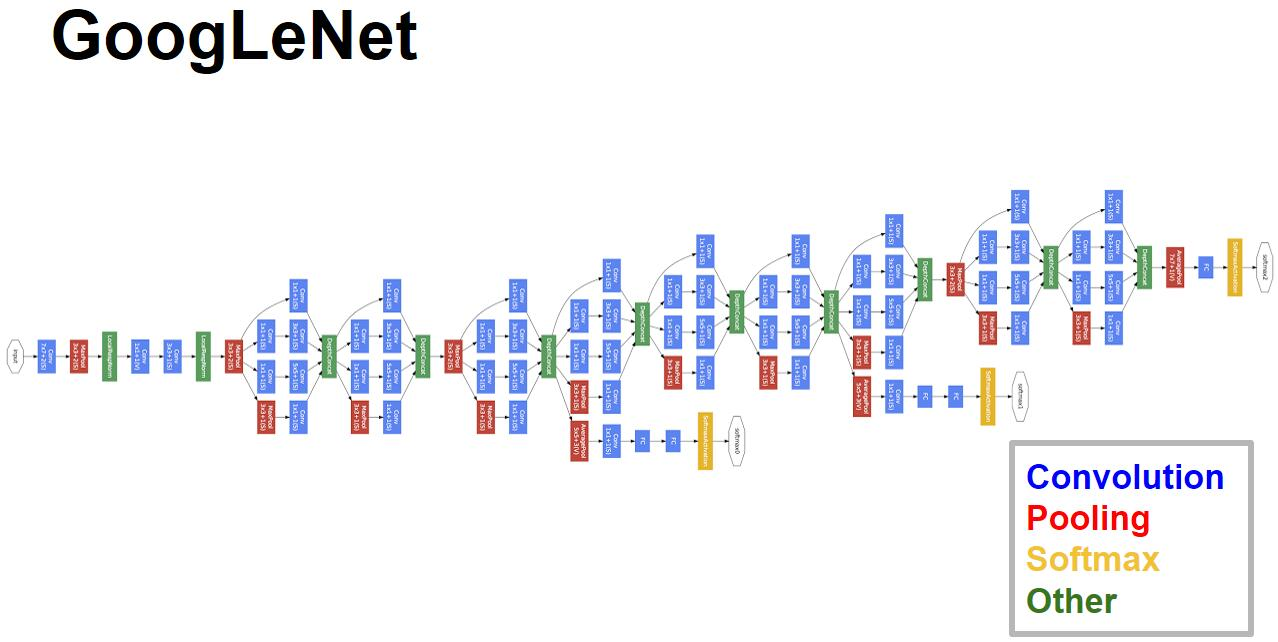
\includegraphics[width=0.7\linewidth]{img/02-10} \end{center}

\hspace{0pt}GoogLeNet相比于以前的卷积神经网络结构,除了在深度上进行了延伸,还对网络的宽度进行了扩展,整个网络由许多块状子网络的堆叠而成,这个子网络构成了Inception结构。上图Inception的四个版本:\(Inception_{v1}\)在同一层中采用不同的卷积核,并对卷积结果进行合并;\(Inception_{v2}\)组合不同卷积核的堆叠形式,并对卷积结果进行合并;\(Inception_{v3}\)则在\(v_2\)基础上进行深度组合的尝试;\(Inception_{v4}​\)结构相比于前面的版本更加复杂,子网络中嵌套着子网络。

\begin{center}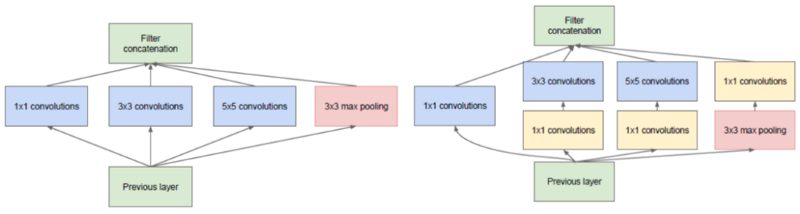
\includegraphics[width=0.7\linewidth]{img/02-11} \end{center}

\begin{center}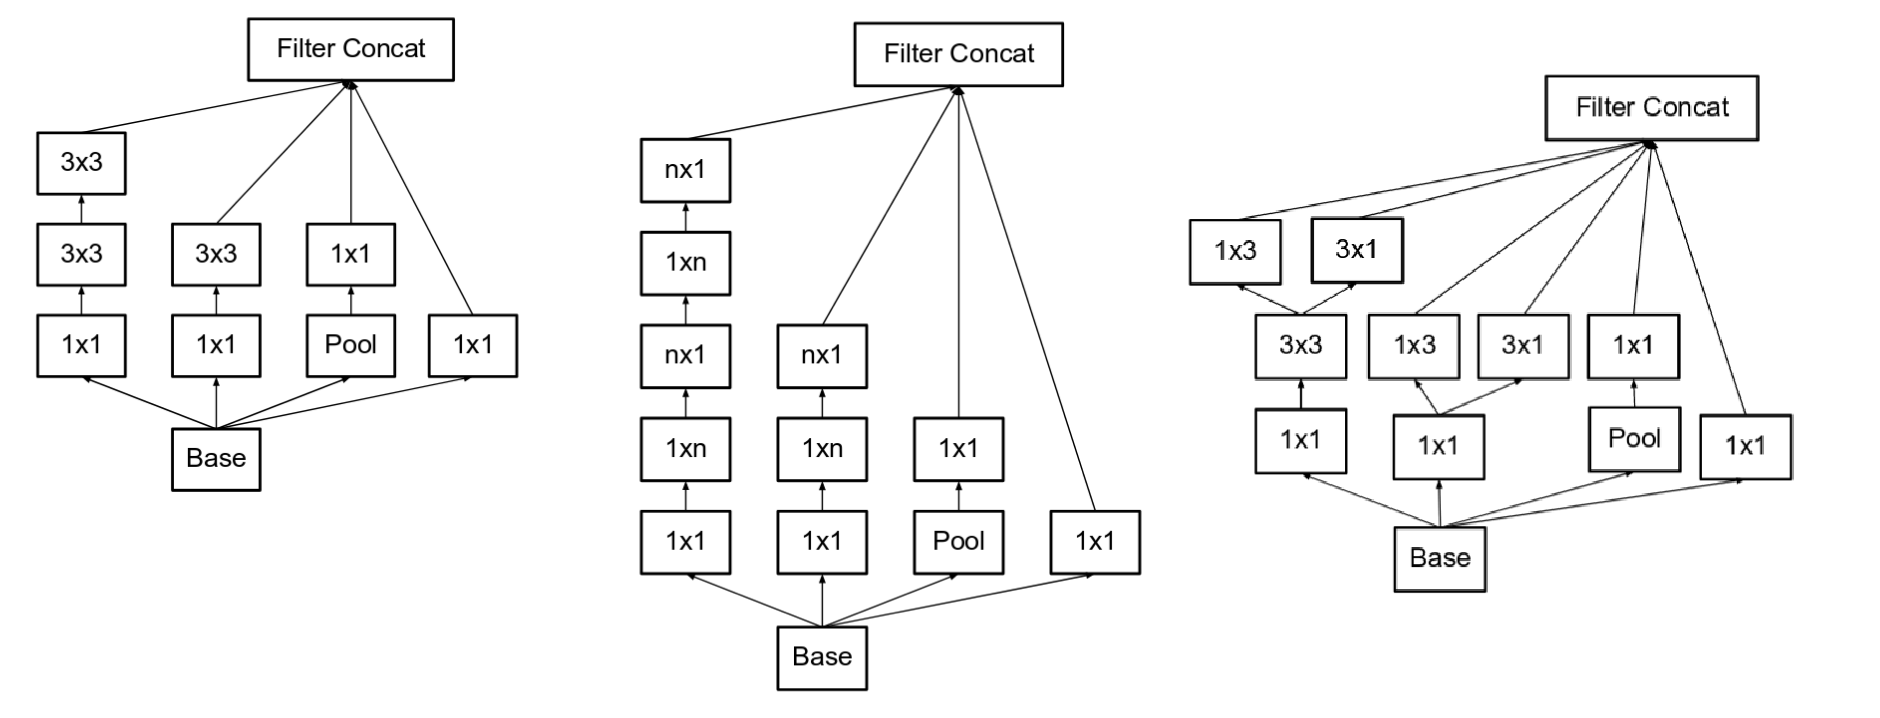
\includegraphics[width=0.7\linewidth]{img/02-14} \end{center}

\begin{center}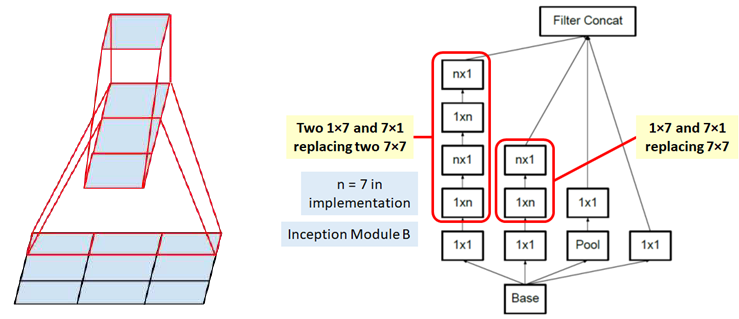
\includegraphics[width=0.7\linewidth]{img/02-12} \end{center}

\begin{center}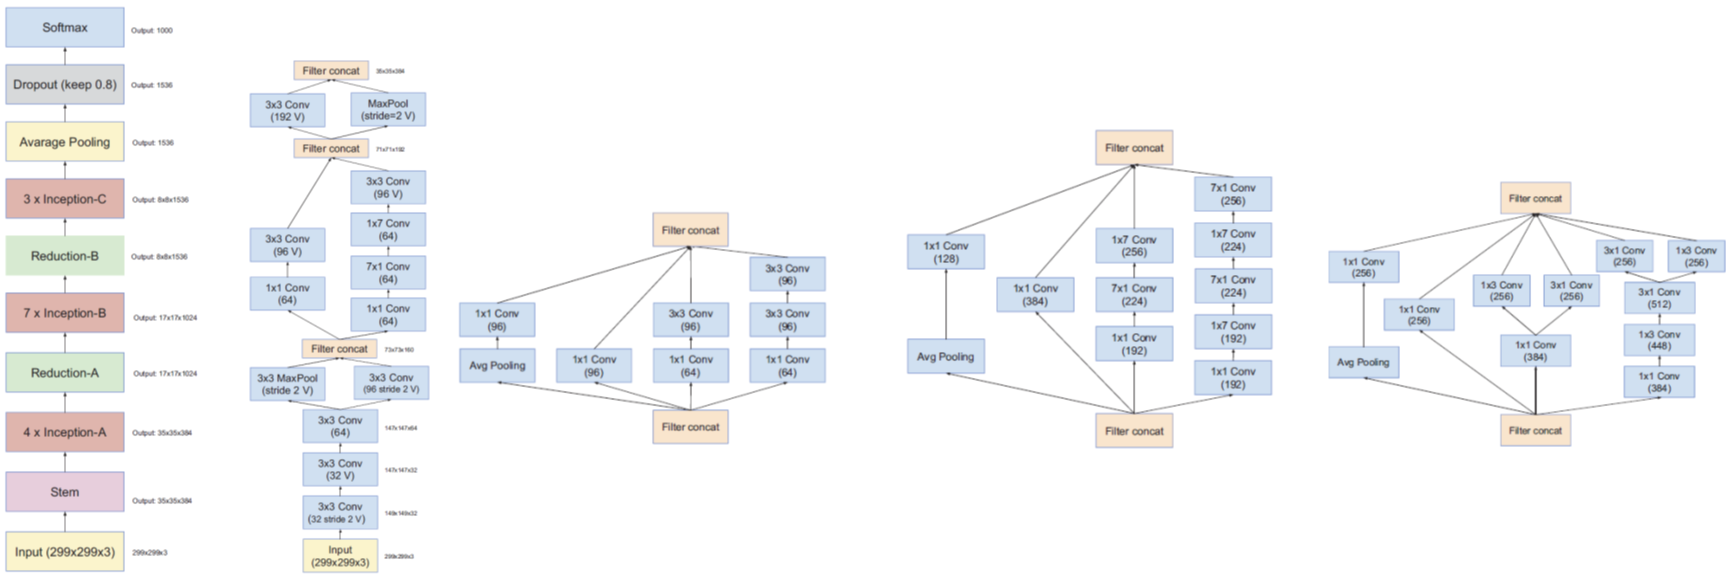
\includegraphics[width=0.7\linewidth]{img/02-13} \end{center}

\begin{longtable}[]{@{}ccccc@{}}
\toprule
\begin{minipage}[b]{0.17\columnwidth}\centering
网络层\strut
\end{minipage} & \begin{minipage}[b]{0.17\columnwidth}\centering
输入尺寸\strut
\end{minipage} & \begin{minipage}[b]{0.17\columnwidth}\centering
核尺寸\strut
\end{minipage} & \begin{minipage}[b]{0.17\columnwidth}\centering
输出尺寸\strut
\end{minipage} & \begin{minipage}[b]{0.17\columnwidth}\centering
参数个数\strut
\end{minipage}\tabularnewline
\midrule
\endhead
\begin{minipage}[t]{0.17\columnwidth}\centering
卷积层\(C_{11}\)\strut
\end{minipage} & \begin{minipage}[t]{0.17\columnwidth}\centering
\(H\times{W}\times{C_1}\)\strut
\end{minipage} & \begin{minipage}[t]{0.17\columnwidth}\centering
\(1\times1\times{C_2}/2\)\strut
\end{minipage} & \begin{minipage}[t]{0.17\columnwidth}\centering
\(\frac{H}{2}\times\frac{W}{2}\times{C_2}\)\strut
\end{minipage} & \begin{minipage}[t]{0.17\columnwidth}\centering
\((1\times1\times{C_1}+1)\times{C_2}\)\strut
\end{minipage}\tabularnewline
\begin{minipage}[t]{0.17\columnwidth}\centering
卷积层\(C_{21}\)\strut
\end{minipage} & \begin{minipage}[t]{0.17\columnwidth}\centering
\(H\times{W}\times{C_2}\)\strut
\end{minipage} & \begin{minipage}[t]{0.17\columnwidth}\centering
\(1\times1\times{C_2}/2\)\strut
\end{minipage} & \begin{minipage}[t]{0.17\columnwidth}\centering
\(\frac{H}{2}\times\frac{W}{2}\times{C_2}\)\strut
\end{minipage} & \begin{minipage}[t]{0.17\columnwidth}\centering
\((1\times1\times{C_2}+1)\times{C_2}\)\strut
\end{minipage}\tabularnewline
\begin{minipage}[t]{0.17\columnwidth}\centering
卷积层\(C_{22}\)\strut
\end{minipage} & \begin{minipage}[t]{0.17\columnwidth}\centering
\(H\times{W}\times{C_2}\)\strut
\end{minipage} & \begin{minipage}[t]{0.17\columnwidth}\centering
\(3\times3\times{C_2}/1\)\strut
\end{minipage} & \begin{minipage}[t]{0.17\columnwidth}\centering
\(H\times{W}\times{C_2}/1\)\strut
\end{minipage} & \begin{minipage}[t]{0.17\columnwidth}\centering
\((3\times3\times{C_2}+1)\times{C_2}\)\strut
\end{minipage}\tabularnewline
\begin{minipage}[t]{0.17\columnwidth}\centering
卷积层\(C_{31}\)\strut
\end{minipage} & \begin{minipage}[t]{0.17\columnwidth}\centering
\(H\times{W}\times{C_1}\)\strut
\end{minipage} & \begin{minipage}[t]{0.17\columnwidth}\centering
\(1\times1\times{C_2}/2\)\strut
\end{minipage} & \begin{minipage}[t]{0.17\columnwidth}\centering
\(\frac{H}{2}\times\frac{W}{2}\times{C_2}\)\strut
\end{minipage} & \begin{minipage}[t]{0.17\columnwidth}\centering
\((1\times1\times{C_1}+1)\times{C_2}\)\strut
\end{minipage}\tabularnewline
\begin{minipage}[t]{0.17\columnwidth}\centering
卷积层\(C_{32}\)\strut
\end{minipage} & \begin{minipage}[t]{0.17\columnwidth}\centering
\(H\times{W}\times{C_2}\)\strut
\end{minipage} & \begin{minipage}[t]{0.17\columnwidth}\centering
\(5\times5\times{C_2}/1\)\strut
\end{minipage} & \begin{minipage}[t]{0.17\columnwidth}\centering
\(H\times{W}\times{C_2}/1\)\strut
\end{minipage} & \begin{minipage}[t]{0.17\columnwidth}\centering
\((5\times5\times{C_2}+1)\times{C_2}\)\strut
\end{minipage}\tabularnewline
\begin{minipage}[t]{0.17\columnwidth}\centering
下采样层\(S_{41}\)\strut
\end{minipage} & \begin{minipage}[t]{0.17\columnwidth}\centering
\(H\times{W}\times{C_1}\)\strut
\end{minipage} & \begin{minipage}[t]{0.17\columnwidth}\centering
\(3\times3/2\)\strut
\end{minipage} & \begin{minipage}[t]{0.17\columnwidth}\centering
\(\frac{H}{2}\times\frac{W}{2}\times{C_2}\)\strut
\end{minipage} & \begin{minipage}[t]{0.17\columnwidth}\centering
\(0\)\strut
\end{minipage}\tabularnewline
\begin{minipage}[t]{0.17\columnwidth}\centering
卷积层\(C_{42}\)\strut
\end{minipage} & \begin{minipage}[t]{0.17\columnwidth}\centering
\(\frac{H}{2}\times\frac{W}{2}\times{C_2}\)\strut
\end{minipage} & \begin{minipage}[t]{0.17\columnwidth}\centering
\(1\times1\times{C_2}/1\)\strut
\end{minipage} & \begin{minipage}[t]{0.17\columnwidth}\centering
\(\frac{H}{2}\times\frac{W}{2}\times{C_2}\)\strut
\end{minipage} & \begin{minipage}[t]{0.17\columnwidth}\centering
\((3\times3\times{C_2}+1)\times{C_2}\)\strut
\end{minipage}\tabularnewline
\begin{minipage}[t]{0.17\columnwidth}\centering
合并层\(M\)\strut
\end{minipage} & \begin{minipage}[t]{0.17\columnwidth}\centering
\(\frac{H}{2}\times\frac{W}{2}\times{C_2}(\times4)\)\strut
\end{minipage} & \begin{minipage}[t]{0.17\columnwidth}\centering
拼接\strut
\end{minipage} & \begin{minipage}[t]{0.17\columnwidth}\centering
\(\frac{H}{2}\times\frac{W}{2}\times({C_2}\times4)\)\strut
\end{minipage} & \begin{minipage}[t]{0.17\columnwidth}\centering
\(0\)\strut
\end{minipage}\tabularnewline
\bottomrule
\end{longtable}

\hypertarget{ux6a21ux578bux7279ux6027-4}{%
\subsection{模型特性}\label{ux6a21ux578bux7279ux6027-4}}

\begin{itemize}
\tightlist
\item
  采用不同大小的卷积核意味着不同大小的感受野,最后拼接意味着不同尺度特征的融合;
\item
  之所以卷积核大小采用1、3和5,主要是为了方便对齐。设定卷积步长stride=1之后,只要分别设定pad=0、1、2,那么卷积之后便可以得到相同维度的特征,然后这些特征就可以直接拼接在一起了;
\item
  网络越到后面,特征越抽象,而且每个特征所涉及的感受野也更大了,因此随着层数的增加,3x3和5x5卷积的比例也要增加。但是,使用5x5的卷积核仍然会带来巨大的计算量。 为此,文章借鉴NIN2,采用1x1卷积核来进行降维。
\end{itemize}

\hypertarget{ux4e3aux4ec0ux4e48ux73b0ux5728ux7684cnnux6a21ux578bux90fdux662fux5728googlenetvggnetux6216ux8005alexnetux4e0aux8c03ux6574ux7684}{%
\section{为什么现在的CNN模型都是在GoogleNet、VGGNet或者AlexNet上调整的?}\label{ux4e3aux4ec0ux4e48ux73b0ux5728ux7684cnnux6a21ux578bux90fdux662fux5728googlenetvggnetux6216ux8005alexnetux4e0aux8c03ux6574ux7684}}

\begin{itemize}
\tightlist
\item
  评测对比:为了让自己的结果更有说服力,在发表自己成果的时候会同一个标准的baseline及在baseline上改进而进行比较,常见的比如各种检测分割的问题都会基于VGG或者Resnet101这样的基础网络。
\item
  时间和精力有限:在科研压力和工作压力中,时间和精力只允许大家在有限的范围探索。
\item
  模型创新难度大:进行基本模型的改进需要大量的实验和尝试,并且需要大量的实验积累和强大灵感,很有可能投入产出比比较小。
\item
  资源限制:创造一个新的模型需要大量的时间和计算资源,往往在学校和小型商业团队不可行。
\item
  在实际的应用场景中,其实是有大量的非标准模型的配置。
\end{itemize}


\backmatter
% \printindex

\end{document}
